\documentclass[11pt]{report}
\usepackage{amsmath}
\usepackage{amssymb}
\usepackage{bbm}
\usepackage{graphicx}
\usepackage{tikz}
\usepackage{enumitem}
\usepackage{graphicx}
\usepackage{longtable}
\usepackage{array}
\usepackage{caption}
\usepackage{subcaption}

\newcommand{\ubt}[1]{\textbf{\underline{#1}}}
\newcommand{\sps}{\\[0.2cm]}
\newcommand{\spn}[1]{\\[#1cm]}
\newcommand{\refn}[1]{(\ref{#1})}
\newcommand{\refx}[1]{\refn{eq:#1}}
\newcommand{\bt}[1]{\textbf{#1}}
\newcommand{\dsp}{\displaystyle}
\newcommand{\NI}{\noindent}
%\newcommand{\real}{ \mathbb{R}}
\newcommand{\mbf}[1]{\mathbf{#1}}
\newcommand{\complex}{\mathbb{C}}
\newcommand{\Laplace}{\mathcal{L}}
\newcommand{\ft}{f(t)}
\newcommand{\ftn}[1]{f(#1)}
\newcommand{\ftp}[1]{f^{#1}(t)}
\newcommand{\Fs}{F(s)}
\newcommand{\Fsp}[1]{F^{#1}(s)}
\newcommand{\LaplaceIntegral}{\int_{0}^{\infty}e^{-st}\ft\text{dt}}
\newcommand{\LFn}[1]{\Laplace \sbracket{#1}}
\newcommand{\LFt}{\Laplace \sbracket{\ft}}
\newcommand{\sbracket}[1]{\left[#1\right]}
\newcommand{\example}[1]{\section*{\ubt{Example #1}}}
\newcommand{\property}{\subsubsection{\ubt{Property}}}
\newcommand{\properties}{\subsubsection{\ubt{Properties}}}
\newcommand{\solution}{\subsubsection{\ubt{Solution}}}
\newcommand{\proposition}[1]{\section*{\ubt{Proposition #1}}}
\newcommand{\eg}{\section*{\ubt{Example}}}

\newcommand{\real}{\mathbbm{R}}

\renewcommand{\baselinestretch}{1.5}
\renewcommand{\contentsname}{Table of Contents}


%\setlength{\parindent}{1em}


\begin{document}
	
	%%%%%%%%%%%%%%%%%%%FRONT COVER%%%%%%%%%%%%%%%%%%%
	\addcontentsline{toc}{chapter}{TITLE PAGE}
	\clearpage
	\thispagestyle{empty}
	\begin{center}
		\Large \bt{SOLUTION OF THE THREE-DIMENSIONAL UNSTEADY INCOMPRESSIBLE NAVIER-STOKES EQUATION}
	\end{center}

	\hspace{7cm}
	
	\begin{center}
		\textbf{\textit{BY}}
	\end{center}
	
	\hspace{5cm}
	
	\begin{center}
		\large \textbf{ADETAYO, ADENIYI JOSHUA
			\\
			17/56EB019}
	\end{center}
	
	\hspace{9cm}
	
	\begin{center}
		A PROJECT SUBMITTED TO THE DEPARTMENT OF MATHEMATICS, FACULTY OF PHYSICAL SCIENCES, UNIVERSITY OF ILORIN, ILORIN, KWARA STATE, NIGERIA. IN PARTIAL FULFILMENT OF REQUIREMENTS FOR THE AWARD OF BACHELOR OF SCIENCE (B. Sc.) DEGREE IN MATHEMATICS.
	\end{center}

	\hspace{7cm}
%	
%	\begin{center}
%		IN PARTIAL FULFILMENT OF REQUIREMENTS FOR THE AWARD OF BACHELOR OF SCIENCE (B. Sc.) DEGREE IN MATHEMATICS.
%	\end{center}
%	\hspace{5cm}
%	\\ \\ 
	\begin{center}
		\textbf{November, 2022}
	\end{center}

	\newpage
	\pagenumbering{roman}
	\addcontentsline{toc}{chapter}{CERTIFICATION}
	\section*{\begin{center}\textbf{\Large CERTIFICATION}   \end{center}}
	This is to certify that this project was carried out by \textbf{ADETAYO, Adeniyi Joshua} with Matriculation Number  \bt{17/56EB019} in the Department of Mathematics, Faculty of Physical Sciences, University of Ilorin, Ilorin, Nigeria, for the award of Bachelor of Science (B.Sc.) degree in Mathematics.
	\\
	\\
	................................... \qquad \qquad\qquad\qquad\qquad\qquad...................... \\
	Dr. E. O. Titiloye   \quad\qquad\qquad\qquad\qquad\qquad\qquad\qquad Date\\
	Supervisor\\
	\\
	\\
	\\
	...................................... \qquad\qquad\qquad\qquad\qquad\qquad ......................\\
	Prof. K. Rauf      \qquad\qquad\qquad\qquad\qquad\qquad\qquad\qquad\quad     Date\\
	Head of Department\\
	\\
	\\
	\\
	..................................... \qquad\qquad\qquad\qquad\qquad\qquad .......................\\
	Prof. T. O. Oluyo \quad\qquad\qquad\qquad\qquad\qquad\qquad\qquad         Date\\
	External Examiner 
	
	\newpage
	%%ACKNOLEDGMENTS%%
	\section*{\begin{center}\textbf{\Large ACKNOWLEDGMENTS}\end{center}}
	\addcontentsline{toc}{chapter}{ACKNOWLEDGMENTS} 					
	All praises\\
	
	\NI i
	
	\newpage
	%%DEDICATION%%
	\section*{\begin{center}\textbf{\Large DEDICATION}\end{center}}
	\addcontentsline{toc}{chapter}{DEDICATION}
	I would like to dedicate the project to God, for the grace and faithfulness of God thus far. For His mercies, guidance and protection throughout my years of study.
	
	\newpage
	%%ABSTRACT%%
	\section*{\begin{center}\textbf{\Large ABSTRACT}\end{center}}
	\addcontentsline{toc}{chapter}{ABSTRACT}
	In this project, we compute the numerical solution of a 3-dimensional Unsteady Incompressible Navier-Stokes Equation using the finite difference method to achieve the space discretization of the equation in a generalized coordinate system.
	
	\newpage
	%%%%%%%%%%%%%%%%%%%TABLE OF CONTENTS%%%%%%%%%%%%%%%%%%%
	\addcontentsline{toc}{chapter}{TABLE OF CONTENTS}
	\tableofcontents
	 \NI I want to give thanks and praises to Almighty God for His loving kindness and mercy for giving me the courage and determination to complete this research work.\\
	
	\NI My profound gratitude and appreciation goes to my supervisor Dr. E. O. Titiloye for his useful and the valuable contribution, correction, and suggestion that greatly helps to the successful completion of this project.\\
	
	\NI My appreciation goes to my amiable and relentless Head of Department Prof. K. Rauf and my amiable Level Adviser, Dr. K.A. Bello for their words of encouragement, concern and support.\\
	
	\NI Also, my appreciation goes to all my esteem Lecturers: Prof. J. A. Gbadeyan, Prof. T. O. Opoola, Prof. O. M. Bamigbola, Prof. M. O. Ibrahim, Prof. O. A. Taiwo, Prof. R. B. Adeniyi, Prof. M. S. Dada, Prof. K. O. Babalola, Prof. A. S. Idowu, Prof. Olubunmi A. Fadipe-Joseph, Dr. Yidiat O. Aderinto, Dr. Catherine N. Ejieji, Dr. B. M. Yisa, Dr. J. U. Abubakar, Dr. Gatta. N. Bakare, Dr. Idayat F. Usamot, Dr. B. M. Ahmed, Dr. O. T. Olootu, Dr. O. A. Uwaheren, Dr. T. L. Oyekunle, Dr. O. Odetunde, Dr. A. Y. Ayinla and all other members of staff of the department of mathematics, who contributed greatly to my academic excellence, obtained during my period of study in the department. May God bless them all.\\
	
	\NI Furthermore, I want to say a big thank you to my family, my sisters, my aunts and uncle, the Obadina family and the Olajumokes \& Adesanyas for the love and support. Sincere appreciation to the families who took me as their own, the Eniwaye's family and Okeneye family, and to my support system my friends who became family; Praise, Wizzy, Orims, Moh, Timilehin, James, Bunmi, Adeola, Feranmi, Janet, Majoti, Mayowa, Emafe, Shiwill, my kolony brothers, Precious, and my fellow coursemates. Gracias muchas. 
	
	
	
	
	\newpage
	\pagenumbering{arabic}
	%%%%%%%%%%%%%%%%%%%CHAPTER ONE%%%%%%%%%%%%%%%%%%%
	\chapter{GENERAL INTRODUCTION}
	Mathematics sometimes referred to the ``backbone`` of science, this argument stems from the fact that mathematical conclusions are frequently applied to other fields of study. As a result, it should come as no surprise that mathematicians are constantly on the lookout for novel ways to solve issues that arise in everyday life.\\
	
	Various technical advancements and scientific discoveries characterized today's globe. As a result, new developments and changes can be seen throughout the field of science. To help enable such developments, scientists in several fields are working on new ways for solving problems that arise in various fields of study.\\
	
	Various properties influence fluid mobility in the physical environment. These qualities must be clearly described in order to offer a transition between the physical and numerical domains in order to bring the behaviour of fluid flow to light and develop a mathematical model. The primary parameter that should be evaluated simultaneously when conducting a flow flow analysis are velocity, pressure, temperature, density and viscosity. These quantities vary depending on physical phenomena such as combustion, multiphase flow, turbulence, mass transport, and so on, and can be classified into kinematic, transport, thermodynamics and other miscellaneous properties.\\
	
	The Navier Stokes equation are non-linear partial differential equation which describes the motion of viscous fluid substances.\\
	
	Also, the Navier Stokes equation can be defined as a partial differential equation that describes the flowing incompressible fluids. The equation is a generalization of the equation devised by the Swiss mathematician Leonhard Euler in the 18th century to described the flow of incompressible and frictionless fluids.\\
	
	The Navier Stokes equation named after the French engineer and physicist Clande-Louis Navier(1785-1836) and Anglo-Irish physicist and mathematician George Gabriel Stokes.\\
	
	The equations were developed over several decades of progressively building the theories, the initial appropriate description of the viscous fluid motion had been indicated in the paper ``principla``\\
	
	Isaace Newton (1687) in which dynamics behaviour because they describe the physics of numerous events of scientific and engineering interests, the Navier-Stokes equations are valuable. They can simulate weather, ocean current, water flow in a pipe, and air reduced forms, the Navier-Stokes equation and in the design of aircraft and auto-mobiles, the study of blood flow, the design of power plants, pollution studies, and many other things. They can be used to model and investigate magnetohydrodynamics when combined with Maxwell's equations.\\
	
	In a purely mathematical sense, the Navier-Stokes equations equally fascinating, the equations are widely used in science and engineering. However, despite the widespread application, their complicated mathematical form mostly restricts engineers to the numerical solutions of these equations.\\
	
	The mathematical proof of the existence of a global smooth solution of the Navier-Stoke equation exists in three dimensions i.e they are infinitely differentiable(or even just bounded) at all points in the domain. This is called the Navier-Stokes existence and smoothness problem. The Clay-mathematics Institute has called it one of the seven most important open problems in mathematics, referred to as the millennium problems and has offered a US \$1 million dollars prize for a solution or a counterexample.
	
	of fluids under constant viscosity was investigated. Later, Daniel Bernoulli (1738) and Swiss mathematician Leonhard Euler (1755) subsequently derived the equation of inviscid flow which is now expressed as Euler's inviscid equations. Euler considered the fluid as a continum allowing him to derive government equations for the motion of inviscid fluids based on differential calculus. His equations were the first written down non-linear partial differential equation.\\
	
	Claude-Louis Navier (1827), Augustin-Louis Cauchy (1828), Simeon Denis Poisson (1829) and Adhimar St. Veriant (1843) investigated the mathematical model of fluid flow, but they overlooked the viscous (frictional) force.\\
	
	Sir George Gabriel Stokes calculated the equation of a viscous flow by adding Newtonian viscous components in 1845, giving rise to the Navier-Stokes Equations, which have been used to generate numerical solution for fluid flow ever since.\\
	
	The Navier-Stokes equations differ from the closely related Euler equations in that they account for viscosity, whereas the Euler equations exclusively simulate inviscid flow. As a result, the Navier-Stokes equation is a parabolic equation, which means that superior analytic features but less mathematical structures (e.g. they are never completely integrable).

	\section{Aim and Objectives}
	The aim of this project is to solve the Navier-Stokes equation for 3-dimensional unsteady incompressible Navier-Stokes Equation using the numerical method of finite difference in a generalizer coordinate system. To an explicit time discretization is added an implicit technique. The Pressure equation is solved by minimizing a discrete norm of the velocity divergence. The method is applied to study the flow around an impulsively started circular cylinder. The time discretization used is an Adams-Bashforth Scheme for the convecture term and the Euler Scheme for the diffusive term.\\
	
	An example of results obtained with this method is presented in this paper; it is related to the computation of the flow around a circular cylinder between two walls.



	\section{Scope of the study}
	Mathematics is a course which is categorised based in individual fields, parts of which is numerical analysis. In this study, we shall consider a discussion on types of fluids, fluid flow and the application of finite difference methods as a numerical approach to solving a three dimensional Navier Stoke equation of unsteady incompressible flow using a stated boundary condition.
	
	
	\section{Significance of study}
	The Navier-Stokes equations are widely used in science and engineering. However, the complicated mathematical form mostly restricts engineers to the numerical solutions of these equations. Numerical solutions for incompressible unsteady viscous flow are of great interest in fluid mechanics for a complex configuration, a good representation of the physics of the flow requires the use of accurate methods using the least amount of computing time. \\
	
	\NI The study help improve:
	\begin{enumerate}
		\item The benefits/uses of the Navier-Stokes equations and fluid mechanics problems e.g the model of weather, ocean currents, water flow in a pipe, blood flow, flow around airfoil (wing)
		
		\item Using a higher order finite difference approximation in space
		
		\item Introducing better adapted boundary conditions especially on the external downstream boundary.
	\end{enumerate}
	

	\section{Basic Notations}
	$P$ = Pressure\\
	$\rho$ = Density \\
	$\vec{U}$ = Fluid Velocity Vector\\
	$V$ = Kinematic Viscosity\\
	$\nabla^2$ = Laplacian Operator\\
	$m$ = mass\\
	$t$ = time\\
	$\nabla$ = gradient differential operator\\
	$u,v,w$ = components of velocity\\
	$x,y,z$ = coordinates\\
	$g$ = gravitational acceleration\\
	$a$ = acceleration\\
	$R_c$ = Reynold's number

	
	%%%%%%%%%%%%%%%%%%%CHAPTER TWO%%%%%%%%%%%%%%%%%%%
	\chapter{FLUIDS}
	\section{Introduction}
	In physics, a fluid is a liquid, gas or other material that continuously deforms (flows) under an applied shear stress, or external force. They have zero shear modulus or, in simple term, are substances, which cannot resist any shear force applied to them.\\
	
	Although, liquids and gases share many qualities in common, yet they also have their own unique characteristics. A gas can be compressed easily, whereas liquids cannot. A given mass of liquid occupies a fixed volume regardless of the container's size and shape; whereas, a gas has no fixed volume and will expand indefinitely unless constrained by the containing vessel.
	
	\section{Types of Fluid}
	\begin{itemize}[label=--]
		\item \bt{Ideal Fluid:} A fluid which is incompressible in nature and has no viscosity falls in the category of an ideal fluid. In practical, Ideal fluid is not found in reality so it is termed as an imaginary fluid since all the fluid that exist in the environment have some viscosity. There is no ideal fluid in reality.
		
		\item \bt{Real Fluid:} A fluid which possesses some viscosity, surface tension and compressibility, is termed as real fluid. Actually, all the fluids existing or present in the environment are called real fluids. Some of the examples are Petrol, Kerosene, ant, etc.
		
		\item \bt{Newtonian Fluids:} If a real fluid obeys the Newton's law of viscosity i.e the shear stress is directly proportional to the shear strain or velocity gradient then it is known as a Newtonian fluid. For a Newtonian fluid, viscosity totally depends upon the temperature and pressure of the fluid. Examples: water, air, air, emulsion, hydrogen, etc.
		
		\bt{Characteristics of Newton Fluid}
		\begin{itemize}[label=*]
			\item Newtonian fluid to not have any elastic properties
			\item They are incompressible, isotropic and unreal
			\item Viscosity is temperature dependent
			\item Viscosity further depends on the various pressures at which it is found
			\item At a fixed temperature, their viscosity remains constant
			\item With the increase in the temperature of a fluid, the viscosity decreases.
			\item The viscosity of this type of fluid is inversely proportional to the increase in the temperature.
			\item The Newtonian fluid was named after Sir Isaac Newton who defined it as a viscous flow
			\item This comply with Newton's law of viscosity
		\end{itemize}
	
		\item\bt{Non-Newtonian Fluid:} Non-Newtonian fluids are the fluids that do not obey Newton's law of viscosity. In other words, a real fluid in which shear stress is not directly proportional to the rate of shear strain is known as Non-Newtonian fluid. Examples: Flubber, Ooblack.\\
		Non-Newtonian fluids can further be classified as:
		\begin{itemize}
			\item \bt{Time dependent fluids:} These fluids are the one for whose shear stress or viscosity decreases with time due to isothermal conditions and steady shear are known as thicotropic and those that increase with time under some circumstances are known as Rheagectic or Antiethicotropic
			
			\item \bt{Time independent fluids:} These fluids are the ones for which the rate of shear at a given point depends on the instantaneous shear stress at the point. These are also known as None-Newtonian viscous fluids or purely viscous fluids. They are further of two types:
			\begin{itemize}
				\item Fluid with yield stress
				\item fluid without yield stress; these also have two kinds:
				\begin{itemize}
					\item Pseudo plastic fluids
					\item dilated fluids
				\end{itemize}
			\end{itemize}
		\end{itemize}
	
		\item \bt{Visco-elastic fluids:} These are fluid formed by a viscous component and an elastic one. For short, viscoelatic fluid are the blend of a solvent and some polymer. Examples are Partes DNA suspensions, various biological fluids and other chemical products.
		
		\item\bt{Ideal Plastic Fluid:} Ideal plastic fluid is a fluid, the shear stress is proportional to the rate of shear strain and in which shear stress is more than the yield value is known as Ideal Plastic fluid. E.g toothpaste can be considered as ideal plastic fluid.
		
		\item\bt{Compressible Fluids:} When density of the fluid changes with the application of external force; it is known as compressible fluid. Density and viscosity is different.
		
		\item\bt{Incompressible Fluids:} In fluid dynamics, an incompressible fluid is a fluid whose density is constant. It is the same throughout space and it does not change throughout. According to the continuity equation, also implies $\rho=0$. It is an idealization used to simplifying analysis. In reality, all fluid are compressible to some extent.
	\end{itemize}

	\section{Properties of Fluids}
	The following properties of fluids are of great importance to the study of fluid mechanics.
	\begin{itemize}[label=--]
		\item \bt{Density:} This is defined as mass per unit volume. The symbol most often used is the Greek letter rho $\rho$. The SI unit of density is $kg/m^3$ i.e $\rho = \frac{m}{v}$.
		
		\item \bt{Surface Tension:} This is a property of the surface of a liquid that allows it to resist on external force. Surface tension has the expression of force per unit length or of energy per unit area. The SI unit is $kg/m^2$
		
		\item \bt{Vapour Pressure or equilibrium vapour pressure: } This is the pressure of a vapour in thermodynamic equilibrium with the condense phases in a closed system.\\
		Vapour pressure is measured in the standard units of pressure. The SI recognises Pressure as a derived unit with the dimension of force per area. SEDFD designates the pascal (pa) as its standard unit. One pascal is one Newton per square meter ($N/m^2$ or $kg/m/s^2$)
		
		\item \bt{Specific Volume:} This is defined as volume per unit mass of a fluid. It is denoted by $V$, given as $V=\frac{v}{m} = \frac{1}{\rho}$
		
		\item \bt{Viscosity:} This is defined as the property of a fluid which determines its resistance to shearing stress.
		
		\item \bt{Pressure:} It is the term used in fluids which is analogues to the term stress used in solids. The pressure of a fluid is the force applied by it per unit area denoted by $P$, $P = \frac{\text{force}}{\text{Area}}$. SI unit of Pressure, $Nm^{-2}$.
		
		\item \bt{Compressibility and Bulk Modulus:} All materials, whether solid, liquid, or gases, are compressible, i.e the volume $V$ of a given mass will be reduced to $V-\delta V$ when a force is exerted uniformly all over its surface. If the forcer per unit area of surface increases from $P$ to $P+\delta P$, the relationship between change of Pressure and change of Volume depends on the bulk modulus of the material,
		\begin{eqnarray*}
			\text{Bulk modulus} = \frac{\text{Change in Pressure}}{\text{Volumetric Strain}}
		\end{eqnarray*}
	
		\item \bt{Capillarity: } If a force tube opens at both ends in lowered vertically into a liquid which wets the tube, the level of the liquid does not wet the tube, the level of liquid in the tube will be depressed below the level of the free surface outside.\\
		Capillarity action is a serious source of error in reading liquid levels in fine gauge tubes particularly as the degree meeting end. Therefore, the contact angle $\theta$ will affected by the cleanliness of the surfaces in contact.
	\end{itemize}
	
	\section{Types of Fluid Flow}
	Fluid flow is a part of fluid mechanics and deals with fluid dynamics. It involves the motion of a fluid subjected to unbalanced forces. This motion continues as long as unbalanced forces are applied.\\
	For example, if you are pouring water from a mug, the velocity of water is very high over the lip, moderately high approaching the lip, and very low at the bottom of the mug. The unbalanced force is gravity, and the flow continues as long as the water is available and the mug is tilted.\\
	
	Fluid flow can be constant or erraties, compressible or incompressible, viscous or non-viscous, to name few characteristics. Some of these qualities are related to the liquid's properties, while others are concerned with the fluid's movement.
	\begin{itemize}[label=--]
		\item \bt{Steady and Unsteady Flow:} The steady flow in which the velocity, pressure, and density are constant at any point with respect to time i.e $\frac{\partial V}{\partial t} = 0,~~ \frac{\partial P}{\partial t}=0,~~ \frac{\partial \rho}{\partial t} = 0$ whereas an unsteady flow is just opposite to steady flow.\sps
		The Unsteady flow is defined as the flow in which the velocity, pressure and density are not constant and it is different with respect to time i.e $\frac{\partial V}{\partial t} \neq 0,~~ \frac{\partial P}{\partial t} \neq 0,~~ \frac{\partial \rho}{\partial t} \neq 0$
		
		\item\bt{Uniform and Non-Uniform Flow:} Uniform flow can be defined as the type of flow in which the velocity does not change with respect to space at any given time. (i.e length of direction of the flow) i.e $\left(\frac{\partial V}{\partial t}\right)$, $t$ is a constant = 0.\sps
		Non-Uniform flow can be defined as the type of flow in which the velocity does changed with respect to space at any given time (i.e length of direction of the flow) i.e  $\left(\frac{\partial V}{\partial t}\right)$, $t$ is a constant $\neq$ 0 
		
		\item\bt{Laminar or Turbulent Flow:} Laminar fluid flow is defined as in which the fluid particles move to streamline or along well-defined paths, which means the flow is straight and parallel is called laminar flows.\sps
		Turbulent fluid flow is defined as in which the fluid particles do not move streamline or along well-defined paths, it flows in a zig-zag way that means the flow is not straight and parallel, it is a zig-zag way and it is called turbulent flow.
		
		\item\bt{Compressible or Incompressible Flow:} Compressible flow can be defined as the flow in which the density is not constant that means from point to point density is changing. Therefore, it is known as compressible flow.
		\begin{eqnarray*}
			\rho \neq \text{ constant}
		\end{eqnarray*}
		Incompressible flow can be defined as the flow in which the density is constant, that means from point to point density is not changing, therefore it is known as incompressible flow.
		\begin{eqnarray*}
			\rho = \text{ constant}
		\end{eqnarray*}
	
		\item\bt{Rotational or Irrotational Flow:} Rotational fluid flow is defined as in which the fluid particles moves to streamline or along well-defined paths, which means the flow is straight and also rotates about its own axis is known as rotational flow.\sps
		Irrotational fluid flow is defined as in which the fluid particles moves to streamline or along well-defined paths, but it does not rotate about its own axis is known as irrotational flow.
		
		\item\bt{One, Two and Three Dimensional Flow:} In one dimensional fluid flow, the name itself indicates fluid is moving in only one dimension (Either $x,y$ or $z$), $u=f(x)$, $V=0$, and $w=0$.\sps
		In two-dimensional fluid flow, the name itself indicates two the fluid is moving in two-dimensions, either $xy, xz$ or $yz$. $u=f_1(x,y),~ v=f_2(x,y)$ and $w=0$.\sps
		In three-dimensional fluid flow, the name also indicate fluid is moving in three dimensions. (either $xyz$, $zyx$ or $yzx$). $u=f_1(x,y,z), v=f_2(x,y,z)$, and $w=f_3(x,y,z)$.
		
		\item \bt{Isothermal Flow:} Is a model of compressible fluid flow whereby the flow remains at the same temperature while flowing in a conduit.
		
		\item\bt{Inviscid Flow:} The flow of a fluid that is assumed to have no viscosity is called an inviscid flow.
		
		\item\bt{Coutte Flow:} This refers to the laminar flow of a viscous fluid in the space between two parallel plates, one of which is moving relative to the other.
		
		\item\bt{Super Fluidity:} This is a state of matter to which the matter behaves like a fluid without viscosity and with infinite thermal conductivity.
		
		\item\bt{Transient Flow:} This is a flow where the velocity and pressure changes overtime.
		
		\item\bt{Transonic Flow:} This refers to the condition of flight in which a range of velocities of a flow exist surrounding and flowing fast an air vehicle or aircraft SERERE concurrently below or above the speed of sound in the range of mack 0.8 to 1.0 at sea level.
	\end{itemize}
	
	
	\section{The Fluid Equations}
	Thermo-fluid ancidents directed by governing equations are based on the laws of conservation. To solve fluid dynamics issues, three conservation rules are used, which can be stated in integral or differential form. The conservation laws can be applied to a control value, which is a section of the flow. A control volume is a discrete space volume in which fluid regarding the content of the problem and are expressed based on the principles of conservation of mass, momentum of  energy:
	\begin{itemize}[label=--]
		\item\bt{Conservation of Mass:} Continuity Equation
		\item\bt{Conservation of Momentum:} Newton's Second Law
		\item\bt{Conservation of energy:} First law of thermodynamic or Energy equation
	\end{itemize}
	The equations of conservation in the Eulerian System in which fluid motion is described and expressed as continuity equation for mass, Navier-Stokes. Equations for momentum and Energy Equation for the first law of thermodynamics.\\
	The equations are all considered simultaneous to examine fluid and flow fields.
	
	\section{Continuity Equation}
	One of the fundamental principles used in the analysis of flows is known as the continuity of flow derived from the fact that mass is always conserved in fluid regardless of the pipeline complexity or direction of flow. The mass in the control volume can neither be created nor destroyed. The conservation of mass states that the mass flow difference throughout the system between inlet and outlet is zero. The equation;
	\begin{eqnarray}
		\frac{\partial \rho}{\partial t} + \nabla \cdot (\rho \vec{V}) = 0 \label{eq:2_1}
	\end{eqnarray}
	or equally,
	\begin{eqnarray}
		\frac{\nabla \rho}{\nabla t} + \rho(\nabla \cdot \vec{V}) = 0 \label{eq:2_2}
	\end{eqnarray}
	where, \\
	\hspace*{1cm} $\rho$ = Density\\
	\hspace*{1cm} $\vec{V}$ = Flow velocity vector field
	Conservative forms of equation can be obtained by applying the underlying physical principle (conservation of mass in this case) to a fluid element found in space. Non-conservative forms are obtained by considering fluid elements moving the flow field.\\
	For incompressible flows, density has a known constant value since it does not change as it moves with the flow and also for incompressible flows, it's not possible to talk about equation of state.
	
	This equation \refx{2_2} is simplified as below, which indicate a steady state process, $\dfrac{\Delta \rho}{\Delta t} = 0$, then 
	\begin{eqnarray*}
		\nabla \cdot \vec{V} = \frac{\partial u}{\partial x} + \frac{\partial v}{\partial y} + \frac{\partial w}{\partial z} = 0
	\end{eqnarray*}
	
	\section{Derivation of the Navier-Stokes Equation}
	\subsection{Cauchy Equation}
	First we derive Cauchy's equation using Newton's Second Law.\\
	We take a differential fluid element. We consider the element as a material element (instead of a control volume) and apply Newton's Second Law
	\begin{eqnarray*}
		F = ma~~;\qquad m \cdot a = \sum \vec{F}
	\end{eqnarray*}
	Since
	\begin{eqnarray*}
		a(t) = \frac{DV(\vec{t})}{Dt},
	\end{eqnarray*}
	we have
	\begin{equation}
		m \cdot \frac{DV(\vec{t})}{Dt} = \sum \vec{F}\tag{1}\label{eq:2_t1_1}
	\end{equation}
	where;\\
	\hspace*{1cm}$m$ = mass\\
	\hspace*{1cm}$a$ = acceleration\\
	\hspace*{1cm}$\sum \vec{F}$ = total force\\
	we express the total force as the sum of body forces and surface forces
	\begin{eqnarray*}
		\sum \vec{F} = \sum \vec{F}_{\text{body}} + \sum \vec{F}_{\text{surface}}
	\end{eqnarray*}
	thus, equation \refx{2_t1_1} can be written as
	\begin{equation}
			m \cdot \frac{DV(\vec{t})}{Dt} = \sum \vec{F}_{\text{body}} + \sum \vec{F}_{\text{surface}}\tag{2}\label{eq:2_t1_2}
	\end{equation}
	{~}\spn{0.4}
	\begin{minipage}{50em}
		\NI\fbox{
			\begin{minipage}{12em}
				Body Force:\\
				Gravity force\\
				Electromagnetic force\\
				centrifugal force\\
				coriolis force\\
			\end{minipage}	
		}\\
		{~}\spn{0.6}
		\NI\fbox{
			\begin{minipage}{12em}
				\NI Surface force:\\
				Pressure forces\\
				viscous forces\\
			\end{minipage}
		}\spn{0.5}
	\end{minipage}
	
	\NI We consider the x-component of equation \refx{2_t1_2}\\
	since $m=\rho dx dy dz$ and $\vec{V} = (u,v,w)$, we have;
	\begin{equation}
		\rho dx dy dz \cdot \frac{DV}{Dt} = \sum \vec{F}_{\text{body}} + \sum \vec{F}_{\text{surface}}\tag{3}\label{eq:2_t1_3}
	\end{equation}
	where $\rho$ is the fluid density\\
	We denote the stress tensor $\sigma_{ij}$ (pressure force + viscous force)
	\begin{eqnarray*}
		\sigma_{ij} = \begin{bmatrix}
			\sigma_{xx} & \sigma_{xy} \sigma_{xz}\sps
			\sigma_{yx} & \sigma_{yy} & \sigma_{yz}\sps
			\sigma_{zx} & \sigma_{zy} & \sigma_{zz}
		\end{bmatrix} \implies \text{stress tensor}
	\end{eqnarray*}
	The viscous stress tensor
	\begin{eqnarray*}
		\tau_{ij} = \begin{bmatrix}
			\tau_{xx} & \tau_{xy} \tau_{xz}\sps
			\tau_{yx} & \tau_{yy} & \tau_{yz}\sps
			\tau_{zx} & \tau_{zy} & \tau_{zz}
		\end{bmatrix} \implies \text{viscous stress tensor}
	\end{eqnarray*}
	The strain (deformation) rate tensor
	\begin{eqnarray*}
		\epsilon_{ij} = \begin{bmatrix}
			\epsilon_{xx} & \epsilon_{xy} \epsilon_{xz}\sps
			\epsilon_{yx} & \epsilon_{yy} & \epsilon_{yz}\sps
			\epsilon_{zx} & \epsilon_{zy} & \epsilon_{zz}
		\end{bmatrix} = 
						\begin{bmatrix}
							\frac{\partial u}{\partial x} & \frac{1}{2}\left(\frac{\partial u}{\partial y} + \frac{\partial v}{\partial x}\right) & \frac{1}{2}\left(\frac{\partial v}{\partial z}+ \frac{\partial w}{\partial x}\right)\sps
							%%%%%%%%%%%%%%%%%%%%%%%%%%%%%%%%%%%%%%
							\frac{1}{2}\left(\frac{\partial v}{\partial x}+ \frac{\partial u}{\partial y}\right) & \frac{\partial v}{\partial y} & \frac{1}{2}\left(\frac{\partial v}{\partial z}+ \frac{\partial w}{\partial y}\right)\sps
							%%%%%%%%%%%%%%%%%%%%%%%%%%%%%%%%%%%%%%%%%
							\frac{1}{2}\left(\frac{\partial w}{\partial x}+ \frac{\partial u}{\partial z}\right) & \frac{1}{2}\left(\frac{\partial w}{\partial y}+ \frac{\partial v}{\partial z}\right) & \frac{\partial w}{\partial z}
						\end{bmatrix}
	\end{eqnarray*}
	
	\NI Now, let $\vec{\tau}_x = (\sigma_{xx}, \sigma_{xy}, \sigma_{xz}),~~ \vec{\tau}_y = (\sigma_{yx}, \sigma_{yy}, \sigma_{yz}),~~ \vec{\tau}_z = (\sigma_{zx}, \sigma_{zy}, \sigma_{zz})$ be stress vectors on the planes perpendicular to the coordinate axes.
	\begin{figure}[!h]
		\centering
		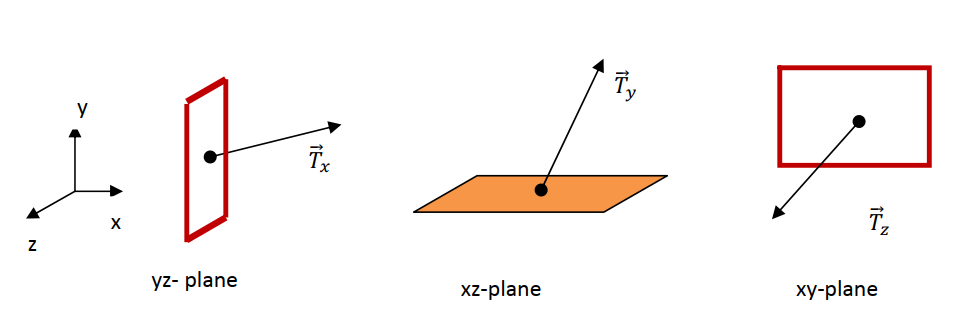
\includegraphics[width=1.02\linewidth]{niyi_img1}
	\end{figure}
	Then the stress vector $\vec{F}$ any point associated with a plane of unit normal vector $\vec{n}=(n_1, n_2, n_3)$ can be expressed as
	\begin{equation}
		\vec{F} = n_1\vec{\tau}_x + n_2\vec{\tau}_y n_3\vec{\tau}_z = (n_1, n_2, n_3) \begin{bmatrix}
			\sigma_{xx} & \sigma_{xy} \sigma_{xz}\sps
			\sigma_{yx} & \sigma_{yy} & \sigma_{yz}\sps
			\sigma_{zx} & \sigma_{zy} & \sigma_{zz}
		\end{bmatrix} \tag{4}\label{eq:2_t1_4}
	\end{equation}
	{~}\sps
	We consider the x-component of the net surface force $\dsp \sum F_{x,\text{surface}}$ using the figure below.
		\begin{figure}[!h]
		\centering
		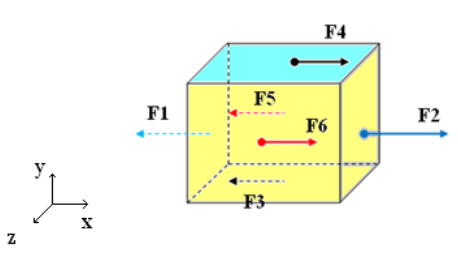
\includegraphics[width=0.9\linewidth]{niyi_img2}
	\end{figure}
	
	Using Taylor's formula we get
	\begin{eqnarray*}
		F_1 = -\left(\sigma_{xx} - \frac{dx}{2}\frac{\partial \sigma_{xx}}{\partial x}\right)dxdz && F_2 = \left(a_{xx}+\frac{dx}{2}\frac{\partial\sigma_{xx}}{\partial x}\right)dxdz\sps
		F_3 = - \left(\sigma_{xx} - \frac{dy}{2}\frac{\partial\sigma_{yx}}{\partial y}\right)dxdy && 	F_3 = \left(\sigma_{xx} + \frac{dy}{2}\frac{\partial\sigma_{yx}}{\partial y}\right)dxdy
	\end{eqnarray*}
	Thus,
	\begin{eqnarray*}
		\sum F_{x,\text{surface}} = F_1 + F_2 + F_3 + F_4 + f_5 + F_6 = \left(\frac{\partial \sigma_{xx}}{\partial x} + \frac{\partial \sigma_{yx}}{\partial y} + \frac{\partial \sigma_{zx}}{\partial z}\right)
	\end{eqnarray*}
	If we assume that the only body force is the gravity force, we have,
	\begin{eqnarray}
		\sum F_{x,body} = m \cdots g_x = \rho \cdot dxdydz \cdot g_x
	\end{eqnarray}
	Now from \refx{2_t1_3}
	\begin{equation}
			\rho dx dy dz \cdot \frac{Du}{Dt} = \sum \vec{F}_{\text{body}} + \sum \vec{F}_{\text{surface}}\tag{3}\label{eq:2_t1_3a}
	\end{equation}
	we have;
	\begin{equation*}
			\rho dx dy dz \cdot \frac{Du}{Dt} =  \rho dx dy dz \cdot g_x + \left(\frac{\partial \sigma_{xx}}{\partial x} + \frac{\partial \sigma_{yx}}{\partial y} + \frac{\partial \sigma_{zx}}{\partial z}\right)dxdydz
	\end{equation*}
	we divided by $dxdydz$ and get the equation for the x-component:
	\begin{eqnarray*}
		\rho\frac{Du}{Dt} = \rho g_x + \frac{\partial \sigma_{xx}}{\partial x} + \frac{\partial \sigma_{yx}}{\partial y} + \frac{\partial \sigma_{zx}}{\partial z}
	\end{eqnarray*}
	Or
	\begin{equation}
		\rho \cdot \left(\frac{\partial u}{\partial t} + u\frac{\partial u}{\partial x} + v\frac{\partial u}{\partial y} + w\frac{\partial u}{\partial z}\right) pg_x +  \frac{\partial \sigma_{xx}}{\partial x} + \frac{\partial \sigma_{yx}}{\partial y} + \frac{\partial \sigma_{zx}}{\partial z} \tag{x} \label{eq:2_t1_x}
	\end{equation}
	{~}\\
	\NI In the similar way we derive the following equations for y-component:
	\begin{equation}
		\rho \cdot \left(\frac{\partial v}{\partial t} + u\frac{\partial v}{\partial x} + v\frac{\partial v}{\partial y} + w\frac{\partial v}{\partial z}\right) pg_y +  \frac{\partial \sigma_{xy}}{\partial x} + \frac{\partial \sigma_{yy}}{\partial y} + \frac{\partial \sigma_{zy}}{\partial z}\tag{y} \label{eq:2_t1_y}
	\end{equation}
	{~}\\
	\NI z-component:
	\begin{equation}
		\rho \cdot \left(\frac{\partial w}{\partial t} + u\frac{\partial w}{\partial x} + v\frac{\partial w}{\partial y} + w\frac{\partial w}{\partial z}\right) pg_z +  \frac{\partial \sigma_{xz}}{\partial x} + \frac{\partial \sigma_{yz}}{\partial y} + \frac{\partial \sigma_{zz}}{\partial z}\tag{z} \label{eq:2_t1_z}
	\end{equation}
	
	\NI The equations \refx{2_t1_x},\refx{2_t1_y}, \refx{2_t1_z} are called \bt{Cauchy's Equation}.
	
	\subsection{The Navier-Stokes Equation}
	When conserving $\dsp \sum F_{x,\text{surface}}$ we can separate x-components of pressure forces and viscous forces:
	\begin{eqnarray*}
		\frac{\partial \sigma_{xx}}{\partial x} = - \frac{\partial P}{\partial x} + \frac{\partial \tau_{xx}}{\partial x}, ~~~ \frac{\partial \sigma_{yx}}{\partial y} = \frac{\partial \tau_{yx}}{\partial y}, ~~~ \frac{\partial \sigma_{zx}}{\partial z} = \frac{\partial \tau_{zx}}{\partial z}
	\end{eqnarray*}
	in the same way, we can change y-component and z-component\\
	y-component:
	\begin{eqnarray*}
		\frac{\partial \sigma_{xy}}{\partial y} = - \frac{\partial P}{\partial y} + \frac{\partial \tau_{yy}}{\partial x}, ~~~ \frac{\partial \sigma_{xy}}{\partial x} = \frac{\partial \tau_{xy}}{\partial x}, ~~~ \frac{\partial \sigma_{zy}}{\partial z} = \frac{\partial \tau_{zy}}{\partial z}
	\end{eqnarray*}
	z-component:
	\begin{eqnarray*}
		\frac{\partial \sigma_{xz}}{\partial x} = \frac{\partial \tau_{xz}}{\partial x}, ~~~ \frac{\partial \sigma_{yz}}{\partial y} = \frac{\partial \tau_{yz}}{\partial y}, ~~~ \frac{\partial \sigma_{zz}}{\partial z} = - \frac{\partial P}{\partial z} +  \frac{\partial \tau_{zz}}{\partial z}
	\end{eqnarray*}
	
	\NI Thus \bt{Cauchy's equations} becomes\\
	x-component;
	\begin{equation*}
		\rho \cdot \left(\frac{\partial u}{\partial t} + u\frac{\partial u}{\partial t} + v\frac{\partial u}{\partial y}+ w \frac{\partial u}{\partial z}\right) = \rho g_x - \frac{\partial P}{\partial x} + \frac{\partial \tau_{xx}}{\partial x} + \frac{\partial \tau_{yx}}{\partial y} + \frac{\partial \tau_{zx}}{\partial z}
	\end{equation*}
	
	\NI y-component
	\begin{eqnarray*}
		\rho \cdot \left(\frac{\partial v}{\partial t} + u\frac{\partial v}{\partial t} + v\frac{\partial v}{\partial y}+ w \frac{\partial v}{\partial z}\right) = \rho g_y - \frac{\partial P}{\partial y} + \frac{\partial \tau_{xy}}{\partial x} + \frac{\partial \tau_{yy}}{\partial y} + \frac{\partial \tau_{zy}}{\partial z}
	\end{eqnarray*}
	
	\NI z-component
	\begin{eqnarray*}
		\rho \cdot \left(\frac{\partial w}{\partial t} + u\frac{\partial w}{\partial t} + v\frac{\partial w}{\partial y}+ w \frac{\partial w}{\partial z}\right) = \rho g_z - \frac{\partial P}{\partial z} + \frac{\partial \tau_{xz}}{\partial x} + \frac{\partial \tau_{yz}}{\partial y} + \frac{\partial \tau_{zz}}{\partial z}
	\end{eqnarray*}
	
	\NI According to the Newton's law of viscosity, the viscous stress components are related (throw a linear combination) to the (first) dynamic viscosity $\mu$ and the second viscosity $\lambda$.
	\begin{equation}
		\tau_{xx} = 2\mu \frac{\partial u}{\partial x} + \lambda div\vec{V},\quad \tau_{xy} = \mu\left(\frac{\partial u}{\partial y}+\frac{\partial v}{\partial x}\right), \quad \tau_{xz} = \mu\left(\frac{\partial u}{\partial z} + \frac{\partial w}{\partial x}\right) \tag{i}\label{eq:2_t2_i}
	\end{equation}
	\begin{equation}
	\tau_{yx} = \mu\left(\frac{\partial u}{\partial y} + \frac{\partial v}{\partial x}\right),\quad \tau_{yy} = 2\mu\frac{\partial v}{\partial y} + \lambda div\vec{V},\quad \tau_{yz} = \mu\left(\frac{\partial v}{\partial z} + \frac{\partial w}{\partial y}\right) \tag{ii}\label{eq:2_t2_ii}
	\end{equation}
	\begin{equation}
		\tau_{zx} = \mu\left(\frac{\partial u}{\partial z} + \frac{\partial w}{\partial x}\right),\quad \tau_{zy} = \mu\left(\frac{\partial v}{\partial z} + \frac{\partial w}{\partial y}\right),\quad \tau_{zz} = 2\mu\frac{\partial w}{\partial y} + \lambda div\vec{V} \tag{iii}\label{eq:2_t2_iii}
	\end{equation}
	We substitute these $\tau_{ij}$ into Cauchy's equations $x,y,z$ we get \bt{The Navier-Stokes Equations for the compressible flow:}\\
	x-component:
	\begin{eqnarray*}
		\rho \cdot \left(\frac{\partial u}{\partial t} + u\frac{\partial u}{\partial x} + v\frac{\partial u}{\partial y} + w\frac{\partial u}{\partial z}\right) &= \rho g_x - \frac{\partial P}{\partial x} + \frac{\partial}{\partial x}\left[2\mu\frac{\partial u}{\partial x} + \lambda div\vec{V}\right] +\\
		 &\frac{\partial}{\partial y}\left[\mu\left(\frac{\partial u}{\partial y} + \frac{\partial v}{\partial x}\right)\right] + \frac{\partial}{\partial z}\left[\mu\left(\frac{\partial u}{\partial z} + \frac{\partial w}{\partial x}\right)\right] 
	\end{eqnarray*}
	y-component:
	\begin{eqnarray*}
		\rho \cdot \left(\frac{\partial v}{\partial t} + u\frac{\partial v}{\partial x} + v\frac{\partial v}{\partial y} + w\frac{\partial u}{\partial z}\right) &= \rho g_y - \frac{\partial P}{\partial y} + \frac{\partial}{\partial x}\left[\mu\left(\frac{\partial u}{\partial y} + \frac{\partial v}{\partial x}\right)\right] + \frac{\partial}{\partial y}\left[2\mu\frac{\partial v}{\partial y} + \lambda div \vec{V}\right] \\ 
		&+\frac{\partial}{\partial z}\left[\mu\left(\frac{\partial v}{\partial z} + \frac{\partial w}{\partial y}\right)\right] 
	\end{eqnarray*}
	z-component
	\begin{eqnarray*}
		\rho \cdot \left(\frac{\partial w}{\partial t} + u\frac{\partial w}{\partial x} + v\frac{\partial w}{\partial y} + w\frac{\partial u}{\partial z}\right) &= \rho g_z - \frac{\partial P}{\partial z} + \frac{\partial }{\partial x}\left[\mu\left(\frac{\partial u}{\partial z} + \frac{\partial w}{\partial x}\right)\right] + \frac{\partial}{\partial y}\left[\mu\left(\frac{\partial v}{\partial z} + \frac{\partial w}{\partial y}\right)\right]\\
		& + \frac{\partial }{\partial z}2\mu\frac{\partial w}{\partial y} + \lambda div\vec{V}
	\end{eqnarray*}
	For an incompressible flow, we have $div\vec{V} = 0$ and hence from \refx{2_t2_i}, \refx{2_t2_ii} and \refx{2_t2_iii}, $\tau_{ij} = 2\mu\epsilon_{ij}$, where $\epsilon_{ij}$ is the strain rate tensor for the velocity field $\vec{V} = (u,v,w)$ in Cartesian coordinates;
	\begin{eqnarray*}
		\tau_{ij} = 2\mu\epsilon_{ij} &=& 2\mu\begin{bmatrix}
			\frac{\partial u}{\partial x} & \frac{1}{2}\left(\frac{\partial u}{\partial y} + \frac{\partial v}{\partial x}\right) & \frac{1}{2}\left(\frac{\partial u}{\partial z} + \frac{\partial w}{\partial x}\right)\spn{0.4}
			%%%%%%%%%%%%%%%%%%%%%%%%%%%%%%%%%%%%%%%%%%%%%%%%
			\frac{1}{2}\left(\frac{\partial v}{\partial x}+\frac{\partial u}{\partial y}\right) & \frac{\partial v}{\partial y}  & \frac{1}{2}\left(\frac{\partial v}{\partial z} + \frac{\partial w}{\partial y}\right)\spn{0.4}
			%%%%%%%%%%%%%%%%%%%%%%%%%%%%%%%%%%%%%%%%%%%%%%%%%%
			\frac{1}{2}\left(\frac{\partial w}{\partial x} + \frac{\partial u}{\partial z}\right) & \frac{1}{2}\left(\frac{\partial w}{\partial y}+\frac{\partial v}{\partial z}\right) & \frac{\partial w}{\partial z}
		\end{bmatrix}\spn{0.6}
		&=& \begin{bmatrix}
			2\mu\frac{\partial u}{\partial x} & \mu\left(\frac{\partial u}{\partial y} + \frac{\partial v}{\partial x}\right) & \mu\left(\frac{\partial u}{\partial z} + \frac{\partial w}{\partial x}\right)\spn{0.4}
			%%%%%%%%%%%%%%%%%%%%%%%%%%%%%%%%%%%%%%%%%%%%%%%%%%%%%
			\mu\left(\frac{\partial v}{\partial x} + \frac{\partial u}{\partial y}\right) & 2\mu\frac{\partial v}{\partial y} & \mu\left(\frac{\partial v}{\partial z} + \frac{\partial w}{\partial y}\right)\spn{0.4}
			%%%%%%%%%%%%%%%%%%%%%%%%%%%%%%%%%%%%%%%%%%%%%%%%%%%%%
			\mu\left(\frac{\partial w}{\partial x}+ \frac{\partial u}{\partial z}\right) & \mu\left(\frac{\partial w}{\partial y}+ \frac{\partial v}{\partial z}\right) & 2\mu\frac{\partial w}{\partial z}
		\end{bmatrix}
	\end{eqnarray*} 
	{~}\\
	\NI In the case when we consider an incompressible, isothermal Newtonian flow (density $\rho$ = constant, viscosity $\mu$ = constant) with a velocity field $\vec{V}=(u(x,y,z), v(x,y,z), w(x,y,z))$. We can simplify the Navier-Stokes equations to this form:\sps
	x-component
	\begin{eqnarray*}
		\rho\left(\frac{\partial u}{\partial t} + u\frac{\partial u}{\partial x} + v\frac{\partial u}{\partial y} + w\frac{\partial u}{\partial z}\right) = - \frac{\partial P}{\partial x} + \rho g_x + \mu\left(\frac{\partial^2 u}{\partial x^2} + \frac{\partial^2 u}{\partial y^2} + \frac{\partial^2 u}{\partial z^2}\right)
	\end{eqnarray*}
	y-component
	\begin{eqnarray*}
			\rho\left(\frac{\partial v}{\partial t} + u\frac{\partial v}{\partial x} + v\frac{\partial v}{\partial y} + w\frac{\partial v}{\partial z}\right) = - \frac{\partial P}{\partial y} + \rho g_y + \mu\left(\frac{\partial^2 v}{\partial x^2} + \frac{\partial^2 v}{\partial y^2} + \frac{\partial^2 v}{\partial z^2}\right)
	\end{eqnarray*}
	z-component
	\begin{eqnarray*}
		\rho\left(\frac{\partial w}{\partial t} + u\frac{\partial w}{\partial x} + v\frac{\partial w}{\partial y} + w\frac{\partial w}{\partial z}\right) = - \frac{\partial P}{\partial z} + \rho g_z + \mu\left(\frac{\partial^2 w}{\partial x^2} + \frac{\partial^2 w}{\partial y^2} + \frac{\partial^2 w}{\partial z^2}\right)
	\end{eqnarray*}
	which can be written in the vector form as
	\begin{eqnarray*}
		\rho \frac{D\vec{V}}{Dt} = -\nabla P + \rho\vec{g} + \mu\nabla^2\vec{V}
	\end{eqnarray*}
	
	
	
	\section{Conservation of Energy}
	Conservation of Energy is the first law of thermodynamics which states that the sum of the work and heat added to the system will result in the increase of the total energy of the system. 
	\begin{eqnarray*}
		\partial E_t = \partial Q + \partial W
	\end{eqnarray*}
	$\partial Q$ - heat added to the system\\
	$\partial W$ - work done on the system\\
	$\partial E_t$ - increment in the total energy of the system\sps
	
	\NI One of the common types of energy equation is
	\begin{eqnarray*}
		\rho\left[\frac{2h}{2t} + \nabla \cdot (hV)\right] = - \frac{\partial P}{\partial t} + \nabla \cdot (k\nabla T) + \phi
	\end{eqnarray*}
	Where;\\
	\hspace*{1cm} $h$- enthalpy\\
	\hspace*{1cm} $k$ - thermal conductivity\\
	\hspace*{1cm} $\dfrac{\partial h}{\partial t}$ - local change with time \\
	\hspace*{1cm} $\nabla \cdot (hV)$ - convective term\\
	\hspace*{1cm} $-\dfrac{\partial P}{\partial t}$ - Pressure work\\
	\hspace*{1cm} $\nabla \cdot (k\nabla T)$ - Heat flux\\
	\hspace*{1cm} $\phi$ - Heat dissipation term\\
	
	
	
	%%%%%%%%%%%%%%%%%%%CHAPTER THREE%%%%%%%%%%%%%%%%%%%
	\chapter{METHODOLOGY}
	\section{Introduction to Non-Dimensionalization}
	Non-dimensionalization can simply be defined as the partial or full removal of physical dimensions from an equation involving physical quantities by a suitable substitution of variables.
	
	\NI I believe that non-dimensionalizing (also known as sealing or normalizing) should be a preliminary step to developing any model. Scaling helps provide better understanding of the physical situation, with the variation in dimension of the parameters involved in the equation. This allows for experiments to be conducted on smaller scale prototypes provided that any physical effects which are not included in the non-dimensionalized equation are unimportant.
	
	\section{Units and Dimension}
	There's a distinction to be made between dimensions and units. A dimension is a non-numerical measure of a physical variable, whereas a unit is a method of assigning a number of measurement to that dimension. For instance, length is a dimension that is measured in feet (ft) or meters (m).
	
	\section{Non-Dimensionalizing Steps}
	To a non-dimensionalize system of equations, one must do the following:
	\begin{enumerate}
		\item Identify all the independent and dependent variables
		\item Replace each of them with a quantity sealed relative to a characteristic unit of measure to be determined.
		\item Divide through by the coefficient of the highest order polynomial or derivative term.
		\item Choose judiciously the definition of the characteristics unit for each variable so that the coefficient of as many terms as possible become 1.
		\item Rewrite the system of equations in terms of the new dimensionless quantities.
	\end{enumerate}
	As an illustrative examples, consider the equation of the oscillation of pendulum.
	\begin{eqnarray*}
		ml\ddot{\theta} + cl\dot{\theta} + mg\sin\theta = F_0\cos wt
	\end{eqnarray*}
	where;\\
	\hspace*{0.4cm} $m$ = mass \qquad \hspace*{0.4cm} $l$ = length of rod \qquad \hspace*{0.4cm} $c$ = function coefficient \qquad \hspace*{0.4cm} $\ddot{\theta}$ = second derivate\qquad\hspace*{0.4cm} $g$= gravity \qquad\hspace*{0.4cm} $F_0$=External force\\
	\hspace*{0.4cm} $w$= frequency\\
	
	\begin{enumerate}
		\item The fundamental unit\spn{0.5}
			\fbox{
			\begin{minipage}{4cm}
				mass (m)\\
				length (l) \\
				time (t) 
			\end{minipage}	
		}
		\item Set; [$ml\ddot{\theta}$] = $mlt^{-2}$ \quad [$F_0$] = $mlt^{-2}$\\
		\hspace*{0.3cm} $[c] = mt^{-1}$\qquad\qquad $[w] = t^{-1}$\\
		\hspace*{0.4cm} $[g] = lt^{-2}$\\
		\hspace*{0.4cm} $ml\ddot{\theta} + cl\ddot{\theta} + mg\sin\theta = F_0\cos wt$
		
		\item The coefficient of the highest ordered term in the front of $\ddot{\theta}$, diving by the $ml$ gives:
		\begin{eqnarray*}
			\ddot{\theta} + \frac{c}{m}\dot{\theta} + \frac{g}{l}\sin \theta = \frac{F_0}{ml}\cos wt
		\end{eqnarray*}
		since $w_0 = \dfrac{1}{t}$, and $g\dfrac{l}{t^2}$, then
		\begin{eqnarray*}
			w_0 = \sqrt{\frac{g}{l}}
		\end{eqnarray*}
		To make time non-dimensional, we make
		\begin{eqnarray*}
			\tau = w_0
		\end{eqnarray*}
		where $\tau$ is dimensionless time
		
		\item Replacing the derivatives, we have
		\begin{eqnarray*}
			\frac{\partial \theta}{\partial t} &=& \frac{\partial \theta}{\partial \tau} \frac{\partial \tau}{\partial t} = w_0\frac{\partial \theta}{\partial \tau}\sps
			\ddot{\theta} &=& w_0^2\frac{\partial^2\theta}{\partial \tau^2}
		\end{eqnarray*}
		Rewriting the equation, we have;
		\begin{eqnarray*}
			w_0^2 \frac{\partial^2\theta}{\partial\tau^2} + \frac{cw_0}{m}\frac{\partial \theta}{\partial \tau} + w_0^2 \sin\theta\frac{F_0}{ml}\cos\left(\frac{w}{w_0}\tau\right)
		\end{eqnarray*}
		\item The final dimensionless equation in this case becomes;
		\begin{eqnarray*}
			\frac{\partial^2 \theta}{\partial \tau^2} + \frac{c}{mw_0}\frac{\partial\theta}{\partial\tau} + \sin\theta = \frac{F_0}{mlw_0^2}\cos\left(\frac{w}{w_0}\tau\right)
		\end{eqnarray*}
		Let; $\dfrac{c}{mw_0}=\alpha$\sps
		$\dfrac{F_0}{mlw_0^2} = \beta $ and $\dfrac{w}{w_0} = \gamma$\sps
		We have; our dimensionless parameter as:
		\begin{eqnarray*}
			\frac{\partial^2\theta}{\partial \tau^2} + \alpha \frac{\partial\theta}{\partial\tau} + \sin \theta = \beta\cos(\gamma\tau)
		\end{eqnarray*}
	\end{enumerate}
	
	\section{Non-Dimensionalization of Navier-Stokes Equation and Derivation of the Reynold's No.}
	\begin{equation*}
		\rho\left(\frac{\partial\vec{u}}{\partial t} + \left(\vec{u}\cdot \vec{\nabla}\right)\vec{v}\right) = -\vec{\nabla}P + \rho \vec{g} + \mu \nabla^2 \vec{u}
	\end{equation*}
	where\\
	$\rho$= fluid density\\
	$P$= Pressure\\
	$\mu$ = fluid viscosity\\
	$\vec{u}$= fluid velocity vector\\
	$g$=gravity\\
	
	\NI\fbox{
		\begin{minipage}{13cm}
			\bt{Note:} this fluid assumed to be incompressible, Newtonian fluid with only gravity as the external force assumed.\\
			
			\NI Also, that there are multiple(s) equations for the Navier-Stokes equation, one for each velocity component.
		\end{minipage}	
	}\sps
	Variables $U_x, U_y, U_z, x,y,z,t$ and $P$\sps
	Dimensionless definitions:
	\begin{gather*}
		\widehat{U}_x = \frac{U_x - U_{xr}}{U_{xs}},\quad \widehat{U}_y = \frac{U_y - U_{xr}}{U_{ys}}, \quad \widehat{U}_z = \frac{U_z - U_{zr}}{U_{zs}},\quad
		\widehat{x} = \frac{x- x_{r}}{x_{s}}, \sps
		 \widehat{y} = \frac{y- y_{r}}{y_{s}},\quad \widehat{z} = \frac{z- z_{r}}{z_{s}},\quad  \widehat{t} = \frac{t- t_{r}}{t_{s}},\quad  \widehat{P} = \frac{P- P_{r}}{P_{s}}
	\end{gather*}
	\begin{enumerate}
		\item Assuming the variables are centred at zero, the reference values can go away, makint it;
		\begin{gather*}
			\widehat{U}_x = \frac{U_x}{U_{xs}},\quad \widehat{U}_y = \frac{U_y}{U_{ys}}, \quad \widehat{U}_z = \frac{U_z}{U_{zs}},\quad
			\widehat{x} = \frac{x}{x_{s}}, \sps
			\widehat{y} = \frac{y}{y_{s}},\quad \widehat{z} = \frac{z}{z_{s}},\quad  \widehat{t} = \frac{t}{t_{s}},\quad  \widehat{P} = \frac{P}{P_{s}}
		\end{gather*}
		
		\item Assuming the velocity and position components are scaled by same amount; $U_s\rightarrow$ velocity components, $L_s\rightarrow$ position components, the variables becomes;
		\begin{gather*}
			\widehat{U}_x = \frac{U_x}{U_{s}},\quad \widehat{U}_y = \frac{U_y}{U_{s}}, \quad \widehat{U}_z = \frac{U_z}{U_{s}},\quad
			\widehat{x} = \frac{x}{L_{s}}, \sps
			\widehat{y} = \frac{y}{L_{s}},\quad \widehat{z} = \frac{z}{L_{s}},\quad  \widehat{t} = \frac{t}{t_{s}},\quad  \widehat{P} = \frac{P}{P_{s}}
		\end{gather*}
	\end{enumerate}
	Rewriting the variables in term of their dimensionless counterparts
	\begin{gather*}
		U_x = U_s\widehat{U}_x, \qquad U_y = U_s\widehat{U}_y, \qquad U_zz = U_s\widehat{U}_z,\qquad x = L_s\widehat{x}\sps
		y = L_s\widehat{y},\qquad  z = L_s\widehat{z}, \qquad t = t_s\widehat{t}, \qquad P = P_s\widehat{P}
	\end{gather*}
	Inputting into the Navier-Stokes Equation
	\begin{equation*}
		\rho\left(\frac{\partial\vec{u}}{\partial t} + \left(\vec{u}\cdot \vec{\nabla}\right)\vec{v}\right) = -\vec{\nabla}P + \rho \vec{g} + \mu \nabla^2 \vec{u}
	\end{equation*}
	{~}\sps
	\NI\fbox{
		\begin{minipage}{13cm}
			\bt{Note:} Since there's only one sealing factor for all the velocity components, the $(U_s)$ stays the same regardless what components we  taking the derivative of. Also, since we are using the same sealing factor for the $(x,y,z)$ variable, we can change $\vec{\nabla}$ to $\dfrac{1}{L_s}\cdot  \vec{\nabla}$
		\end{minipage}	
	}\sps
	
	\begin{eqnarray*}
		\rho\left[\frac{U_s}{t_s}\frac{\partial\widehat{\vec{U}}}{\partial \widehat{t}} + \left( U_s\widehat{\vec{U}} \cdot \frac{1}{L_s}\widehat{\vec{\nabla}}\right)U_s\widehat{\vec{U}}\right] = -\frac{P_s}{L_s}\widehat{\vec{\nabla}}P + \mu\frac{U_s}{L_s^2}\nabla^2\widehat{\vec{U}} + \rho \vec{g}
	\end{eqnarray*}
	Divide by the coefficient of the highest order derivative $\nabla^2$ which is $\mu\dfrac{U_s}{L_s^2}$, we have
	\begin{eqnarray*}
		\frac{\rho L_s^2}{\mu t_s} \frac{\partial \widehat{\vec{U}}}{\partial \widehat{t}} + \frac{\rho U_s L_s}{\mu} \left( \widehat{\vec{U}} \cdot \widehat{\vec{\nabla}} \right)\widehat{\vec{U}} = -\frac{P_sL_s}{\mu U_s}\widehat{\vec{\nabla}}P^2 + \frac{\rho \vec{g}L_s^2}{\mu U_s} + \nabla^2\widehat{\vec{U}}
	\end{eqnarray*}
	we have a dimensionless Navier-Stokes Equation.\sps
	Also, we have $\rho\frac{U_sL_s}{\mu}$ which is the Reynolds number, Re.\sps
	
	\NI Now let set the sealing factor time:
	\begin{eqnarray*}
		t_s = \frac{L_s}{U_s} \implies \frac{\rho L_s^2}{\mu t_s} = \frac{\rho L_s^2}{\mu L_s/U_s} = \frac{\rho U_s L_s}{\mu} = \text{Re}
	\end{eqnarray*}
	If we divide through by the Re, we have
	\begin{eqnarray*}
		\frac{\partial \widehat{\vec{U}}}{\partial \widehat{t}} + \left(\widehat{\vec{U}} \cdot \widehat{\vec{V}}\right)\widehat{\vec{U}} = -\frac{P_s}{\rho U_s^2} \widehat{\vec{V}}\widehat{\rho} + \frac{\vec{g}L_s}{U_s^2} + \frac{\mu}{\rho U_sL_s}\nabla^2 \widehat{\vec{U}}
	\end{eqnarray*}
	we have $\dsp\frac{P_s}{\rho U_s^2}$ which is Euler's number, \bt{Eu}. Also, Froude number which is $\dfrac{U_s}{\sqrt{gL_s}}$, \bt{Fr}. $\dfrac{\vec{g}L_s}{U_s^2}$ can be written as $\dfrac{1}{Fr^2}$.\sps
	We can rewrite the whole equation as
	\begin{eqnarray*}
		\frac{\partial \widehat{\vec{U}}}{\partial \widehat{t}} + \left(\widehat{\vec{U}} \cdot \widehat{\vec{V}}\right)\widehat{\vec{U}} = - Eu\widehat{\vec{\nabla}}\widehat{P} + \frac{1}{Fr^2}\widehat{\vec{g}} + \frac{1}{Re}\nabla^2\widehat{\vec{U}}
	\end{eqnarray*}

	\section{Discretization}
	Discretization is the process of converting continuous functions, models, variables equation into discrete counterparts in applied mathematics.\sps
	This is typically done as a first step towards preparing them for numerical evaluation and implementation on digital computer.\sps
	Dichotomization is a type of discretization in which there are two discrete classes and a continuous variable can be approximated as a binary variable (creating a dichotomy for modelling purposes, as in binary classification)
	
	\section{Finite Difference Method}
	Suppose we are given a table of values $(x_i,y_i), i=0,1,2,\ldots,n$ of a function $y=f(x)$, the values of $x$ being equally spaced, i.e, value of $f(x)$ for some intermediate values of $x$, or to obtain the derivatives of $f(x)$ for some $x$ in the range $x_0 \leq x \leq x_n$.\sps
	Brook Taylor introduced finite differences in 1715, and George Boole (1860), L.M. Malne-Thomson (1933), and Ka roly Jordan have studied them as abstract self-standing mathematical objects(1939). Finite differences can be traced back to just Burgi's (c. 1592) algorithm and work by others, including Isaac Newton. As an alternative to the calculus of infinite simals, the formula calculus of finite differences can be considered.\sps
	A mathematical formula of the type
	\begin{eqnarray}
		f(x+b)-f(x+a)
	\end{eqnarray}
	is known as a finite difference quotient is obtained by dividing a finite difference by $b-a$. The difference operator, usually denoted by $\Delta $ is the operator that maps a function $f$ to the function $\Delta f$ defined by
	\begin{eqnarray}
		\Delta f(x) = f(x+1) - f(x)
	\end{eqnarray}
	Three basic types are commonly considered; forward, backward and central finite difference.\sps
	
	\NI A forward difference denoted $\Delta_h[f]$, of a function $f$ is a function defined as;
	\begin{eqnarray}
		\Delta_h f(x) = f(x+h)-f(x)
	\end{eqnarray}
	
	
	\NI A backward difference uses the function values at $x$ and $x-h$, instead of the values at $x+h$ and $x$, denoted by $\nabla_h[f]$
	\begin{eqnarray}
		\nabla_h f(x)= f(x) - f(x-h) = \Delta_h f(x-h)
	\end{eqnarray}
	
	\NI The central difference is given by
	\begin{eqnarray}
		\delta_h f(x) = f\left(x+\frac{h}{2}\right) - f\left(x-\frac{h}{2}\right) = \Delta_{h/2}f(x) + \nabla_{h/2}f(x)
	\end{eqnarray}
	The derivative of a function $f$ at a point $x$ is defined by the limit
	\begin{eqnarray}
		f'(x) = \lim\limits_{h\to 0}\frac{f(x+h) - f(x)}{h}
	\end{eqnarray}
	
	\NI If $h$ has a fixed value instead of approaching zero, then
	\begin{eqnarray}
		\frac{f(x+h) - f(x)}{h} = \frac{\Delta_h f(x)}{h}
	\end{eqnarray}
		
	\NI If we assume $f$ is twice differentiable, the forward difference divided by $h$, approximating the derivative when $h$ is small
	\begin{eqnarray}
		\frac{\Delta_h f(x)}{h} - f'(x) = O(h) \to 0\quad \text{ as }\quad h \to 0
	\end{eqnarray}
	Applying the same to the backward difference:
	\begin{eqnarray}
			\frac{\nabla_h f(x)}{h} - f'(x) = O(h) \to 0\quad \text{ as }\quad h \to 0
	\end{eqnarray}	
	The center difference, on the other hand, gives a more precise result. If $f$ can be differentiated three times, then
	\begin{eqnarray}
		\frac{\delta_h f(x)}{h} - f'(x) = O(h^2) \label{eq:3_10}
	\end{eqnarray}
	
	\NI We can also obtained the finite difference approximate of the second order derivative and differential operators. Using the central difference formula \refx{3_10} for $\dsp f'(x + \frac{h}{2})$ and $\dsp f'(x - \frac{h}{2})$ we get the central difference approximation of $f$ by using a central difference formula for the derivative of $f'$ at $x$.\sps
	The Second-Order Central difference gives
	\begin{eqnarray}
		f''(x) &=& \frac{\delta^2_h f(x)}{h^2} = \frac{\frac{f(x+h) - f(x)}{h} - \frac{f(x)- f(x-h)}{h}}{h} \notag \sps
		&=& \frac{f(x+h) - 2(fx) + f(x-h)}{h^2}
	\end{eqnarray}
	Applying other differencing formulas similarly in a recursive manner; the second order forward difference gives;
	\begin{eqnarray}
		f''(x) &=& \frac{\Delta_h f(x)}{h^2} = \frac{\frac{f(x+2h)-f(x+h)}{h} - \frac{f(x+h)-f(x)}{h}}{h}\notag\sps
		&=& \frac{f(x+2h) - 2f(x+h)+f(x)}{h^2}
	\end{eqnarray}
	Similarly, the second-order backward gives
		\begin{eqnarray}
		f''(x) &=& \frac{\nabla_h f(x)}{h^2} = \frac{\frac{f(x)-f(x-h)}{h} - \frac{f(x-h) -f(x-2h)}{h}}{h}\notag\sps
		&=& \frac{f(x) - 2f(x-h) + f(x-2h)}{h^2}
	\end{eqnarray}
		
	\NI Finite differences can be applied to multiple variables partial derivatives in many variables are equivalent ot  them. Same partial derivatives are:
	\begin{eqnarray}
		f_x(x,y) &\approx& \frac{f(x+h, y) - f(x-h,y)}{2h}\sps
		f_y(x,y) &\approx& \frac{f(x, y+k) - f(x,y-k)}{2k}\sps
		f_{xx}(x,y) &\approx& \frac{f(x+h,y) - 2f(x,y) + f(x-h,y)}{h^2}\sps
		f_{yy}(x,y) &\approx& \frac{f(x,y+k) - 2f(x,y) + f(x,y-k)}{k^2}\sps
		f_{xy}(x,y) &\approx& \frac{f(x+h, y+k) - f(x+h, y-k) - f(x-h,y+k) + f(x-h, y-k)}{4hk}\label{eq:3_18}
	\end{eqnarray}
	A more efficient formula for \refx{3_18} can be written as
	\begin{eqnarray}
		f_{xy}(x,y) &\approx& \frac{f(x+h, y+k) - f(x+h, y) - f(x,y+k) + 2f(x,y) - f(x-h,y)}{2hk} \notag\sps
		& -& \frac{f(x,y-k) + f(x-h,y-k)}{2hk}\label{eq:3_19}
	\end{eqnarray}

	\section{Implicit and explicit methods}
	Explicit and implicit methods are numerical analytical methodologies for deriving numerical approximations to the solutions of time-dependent ordinary and partial differential equations, as needed in computer simulations of physical processes.\sps
	
	\NI Explicit methods find a solution by solving an equation involving both the current and later states of the system, whereas implicit methods find a solution by solving an equation involving both the current and later states of the system. If you look at it from a mathematical standpoint, $Y(t)$  is the current system state and $Y(t+\Delta t)$ is the state at the later time ($\Delta t$ is a small time step), then, for an explicit method
	\begin{eqnarray}
		Y(t+\Delta t) =F(Y(t))
	\end{eqnarray}
	while for an implicit method one solves an equation
	\begin{eqnarray}
		G(Y(t),Y(t+ \Delta t) ) =0
	\end{eqnarray}
	to find $Y(t+ \Delta t)$.
	
	
	\section{Euler's Method}
	Euler's Method assumes our solution is written in the form of a Taylor's Series. That is, we'll have a function of the form:
	\begin{eqnarray}
		y(x+h) \approx y(x) + hy'(x) + \frac{h^2 y''(x)}{2!} + \frac{h^3 y'''(x)}{3!} + \frac{h^4 y^{iv}(x)}{4!} + \cdots
	\end{eqnarray}
	This gives us a reasonably good approximation if we take plenty of terms, and if the value of $h$ is reasonably small. For Euler's Method, we just take the first 2 terms only.
	\begin{eqnarray}
			y(x+h) \approx y(x) + hy'(x)
	\end{eqnarray}
	The last term is just $h$ times our $\dfrac{dy}{dx}$ expression, so we can write Euler's Method as follows:
	\begin{eqnarray}
		y(x+h) \approx y(x) + hf(x,y)\label{eq:3_24}
	\end{eqnarray}
	
	\NI To use this formula \refx{3_24}, we start with some known value of $y$, which we could call $y_0$. It has this value when $x=x_0$ (We make use of the initial value $(x_0,y_0)$)\sps
	The result of using this formula is the value for $y$, one $h$ step to the right of the current value. Let's call it $y_1$. So we have:
	\begin{eqnarray*}
		y_1 \approx y_0 + hf(x_0,y_0)
	\end{eqnarray*}
	where\\
	$y_1$ is the next estimated solution value;\\
	$y_0$ is the current value;\\
	$h$ is the interval between steps; and \\
	$f(x_0,y_0)$ is the value of the derivative at the starting point, $(x_0,y_0)$.
	
	\NI \bt{Next value:} To get the next value $y_2$, we would use the value we just found for $y_1$ as follows:
	\begin{eqnarray*}
		y_2 \approx y_1 + hf(x_1,y_1)
	\end{eqnarray*}
	We continue this process for as many steps as required.\sps
	
	\NI The right hand of the formula in \refx{3_24} means, ``start at the known $y$ value, then move one step $h$ units to the right in the direction of the slope at that point, which is $\dfrac{dy}{dx}=f(x,y)$. We will arrive at a good approximation to the curve's $y$-value at that new point.''
	
	\eg
	Solve the following initial value problem
	\begin{eqnarray*}
		\frac{dy}{dx} = \frac{y\ln y}{x};\qquad y(2) = e
	\end{eqnarray*}
	
	\solution
	We'll start at the point $(x_0,y_0) = (2,e)$ and use step size of $h=0.1$ and proceed for 10 steps. That is, we''l approximate the solution from $t=2$ to $t=3$ for our differential equation. We'll finish with a set of points that represent the solution, numerically.\sps
	We already know the first value, when $x_0=2$, which is $y_0=e$. We now calculate the value of the derivative at this initial point as
	\begin{eqnarray*}
		\frac{dy}{dx} = f(2,e) = \frac{e\ln e}{2} = \frac{e}{2} \approx 1.3591409
	\end{eqnarray*} 
	This means the slope of the line from $t=2$ to $t=2.1$ is approximately $1.3591409$\sps
	
	\NI Now, for the second step, (since $h=0.1$, the next point is $x+h=2+0.1=2.1$), we substitute what we know into Euler's Method formula \refx{3_24}, and we have:
	\begin{eqnarray*}
		y(x+h)\approx y(x) + hf(x,y)\sps
		y_1 = y(2.1) \approx e+0.1\left(\frac{e}{2}\right) = 2.8541959
	\end{eqnarray*}
	This means the approximate value of the solution when $x=2.1$ is 2.8540959. We'll need the new slope at this point, so we'll know where to head next.
	\begin{eqnarray*}
		\frac{dy}{dx} = f(2.1,2.8541959) = \frac{2.8541959\ln 2.8541959}{2} = 1.4254536
	\end{eqnarray*}
	This means the slope of the approximation line from $x=2.1$ to $x=2.2$ is 1.4254536.
	
	\NI Now, finding the solution value when $x=2.2$, we substitute our known values into the Euler's method, we have
	\begin{eqnarray*}
		y(x+h)\approx y(x) + hf(x,y)\sps
		y(2.2) \approx 2.8540959 + 0.1(1.4254536) = 2.99664126
	\end{eqnarray*}
	Calculating the next new slope at this point, we have
	\begin{eqnarray*}
		f(2.2, 2.99664426) = \frac{2.99664126\ln 2.99664126}{2.2} = 1.49490457
	\end{eqnarray*}
	This means the slope of the approximation line from $x=2.2$ to $x=2.3$ is 1.49480456. The solution value at when $x=2.3$ is given by
	\begin{eqnarray*}
		y(x+h) \approx y(x) + hf(x,y)\sps
		y(2.3) \approx 2.99664126 + 0.1(.149490456) = 3.1461317
	\end{eqnarray*}
	The values up to $x=3$ in the following table. Most of the time, we'll use computers to find these approximation.
	\begin{longtable}{|m{2cm}|m{4cm}|m{4cm}|}
			\hline
			$x$ & $y$ & $\dfrac{dy}{dx}$\\\hline
			2.0 & 2.7182818285 & 1.3591409142\\\hline
			2.1 & 2.8541959199 & 1.4254536226\\\hline
			2.2 & 2.9967412821 & 1.4949999323\\\hline
			2.3 & 3.1462412754 & 1.5679341197\\\hline
			2.4 & 3.3030346873 & 1.6444180873\\\hline
			2.5 & 3.4674764961 & 1.7246216904\\\hline
			2.6 & 3.6399386651 & 1.8087230858\\\hline
			2.7 & 3.8208109737 & 1.8969091045\\\hline
			2.8 & 4.0105018841 & 1.9893756448\\\hline
			2.9 & 4.2094394486 & 2.08632809\\\hline
			3.0 & 4.4180722576 &\\\hline
	\end{longtable}

	
	\section{Adams-Bashforth Methods}
	The Adams-Bashforth methods are explicit methods. The coefficients are $a_{s-1} = -1$ and $a_{s-2} = \cdots = a_0 = 0$, while the $b_j$ are chosen such that the methods have order $s$ (this determines the methods uniquely).\sps
	The Adams-Bashforth method with $s=1,2,3,4,5$ are:
	\begin{eqnarray*}
		y_{n+1} &=& y_n + hf(t_n,y_n),\qquad \text{(This is the Euler method)}\sps
		y_{n+2} &=& y_{n+1} + h\left(\frac{3}{2}f(t_{n+1}, y_{n+1}) - \frac{1}{2}f(t_n, y_n\right)\sps
		y_{n+3} &=& y_{n+2} + h\left(\frac{23}{12}f(t_{n+2}, y_{n+2}) - \frac{16}{12}f(t_{n+1}, y_{n+1}) + \frac{5}{12}f(t_n,y_n)\right)\sps
		y_{n+4} &=& y_{n+3} + h\left(\frac{55}{24}f(t_{n+3}, y_{n+3}) - \frac{59}{24}f(t_{n+2}, y_{n+2}) + \frac{37}{24}f(t_{n+1}, y_{n+1}) - \frac{9}{24}f(t_n,y_n)\right)\sps
		y_{n+5} &=& y_{n+4} + h\left( \frac{1901}{720}f(t_{n+4}, y_{n+4}) - \frac{2774}{720}f(t_{n+3}, y_{n+3}) + \frac{2616}{720}f(t_{n+2}, y_{n+2}) \right.\sps
		&&\left.- \frac{1274}{720}f(t_{n+1}, y_{n+1}) + \frac{251}{720}f(t_n,y_n)
		\right)
	\end{eqnarray*}
	The coefficients $b_j$ can be determined as follows. Use polynomial interpolation to find the polynomial $p$ of degree $s-1$ such that
	\begin{eqnarray*}
		p(t_{n+i}) = f(t_{n+i}, y_{n+i}),\qquad \text{for } i = 0,\ldots, s-1
	\end{eqnarray*}
	The Lagrange formula for polynomial interpolation yields
	\begin{eqnarray*}
		p(t) = \sum_{j=0}^{s-1}\frac{(-1)^{s-j-1}  f(t_{n+j}, y_{n+j})}{j!(s-j-1)!h^{s-1}}\prod_{\substack{i=0\\i\neq j}}^{s-1}(t-t_{n+i})
	\end{eqnarray*}
	The polynomial $p$ is locally a good approximation of the right-hand side of the differential equation $y' = f(t,y)$ that is to be solved, so consider the equation $y' = p(t)$ instead. This equation can be solved exactly; the solution is simply the integral of $p$. This suggests taking 
	\begin{eqnarray*}
		y_{n+s} = y_{n+s-1} + \int_{t_{n+s-1}}^{t_{n+s}}p(t) dt
	\end{eqnarray*}	
	
	\NI The Adams-Bashforth method arises when the formula for $p$ is substituted. The coefficients $b_j$ turn out to be given by
	\begin{eqnarray*}
		b_{s-j-1} = \frac{(-1)^j}{j!(s-j-1)!}\int_{0}^{1}\prod_{\substack{i=0\\i\neq j}}^{s-1}(u+i)du,\qquad \text{for } j=0,\ldots, s-1
	\end{eqnarray*}
	Replacing $f(t,y)$ by its interpolant $p$ incurs an error of order $h^s$, and it follows that the $s$-step Adams-Bashforth method has indeed order $s$.\\
	
	\NI The Adams-Bashforth methods were designed by John Couch Adams to solve a differential equation modelling capillary action due to Francis Bashforth. Bashforth(1883) published his theory and Adams' numerical method (Goldstine 1977).
	
	
	%%%%%%%%%%%%%%%%%%%CHAPTER FOUR%%%%%%%%%%%%%%%%%%%
	\chapter{}
	The basic equations are the three dimensional time-dependent imcompressible Navier-Stokes equations in velocity-pressure formulation with the continuity equation.
	\begin{eqnarray}
		\rho\frac{D\vec{V}}{Dt} = -\vec{V} P + \rho\vec{g} + \mu \Delta^2\vec{V}
	\end{eqnarray}
	which can also be written as
	\begin{eqnarray}
		\rho\left(\frac{\partial \vec{U}}{dt} + (\vec{U}\cdot \vec{\nabla})\vec{V}\right) = -\vec{\nabla}P + \rho\vec{g} + \mu\vec{\nabla}^2\vec{U}
	\end{eqnarray}
	\begin{equation*}
		\frac{\partial\vec{U}}{\partial t} + (\vec{U}\cdot\nabla)\vec{U} = -\vec{\nabla}P + \frac{1}{R_e} \nabla \cdot (\nabla\vec{U})
	\end{equation*}
	where $R_e$ is the Reynold's number. The equation,
	\begin{equation}
		\frac{\partial \vec{U}}{\partial t} + (\vec{U}\cdot\nabla)\vec{U} + \nabla P = \frac{1}{R_e}\nabla\cdot(\nabla\vec{U})\label{eq:4_3}
	\end{equation}
	\begin{equation}
		\nabla \cdot \underline{U} = 0\label{eq:4_4}
	\end{equation}
	is an unbounded/domain $\Omega$ subjected to Dirichlet boundary condition on the body surface $\Gamma$, a free stream condition at affinite
	\begin{eqnarray*}
		\underline{U}(x,t=0) = \vec{U}_0(x), \text{ in } \vec{\Omega} \equiv \Omega + \Gamma,\sps
	\end{eqnarray*}
	The equation \refx{4_3} and \refx{4_4} above now rewritten as follows:
	\begin{gather}
		\frac{\partial U}{\partial t} + \nabla\times\underline{U} + \nabla Q = \frac{1}{R_e}\nabla \cdot (\nabla\underline{U}),\label{eq:4_5}\sps
		\nabla\cdot\underline{U} = 0,\label{eq:4_6}
	\end{gather}
	where 
	\begin{eqnarray*}
		Q = P + \frac{1}{2}\Bigg|\underline{U}\Bigg|^2
	\end{eqnarray*}
	denotes the total pressure.\\
	
	\NI A generalized coordinate system is required for complete configurations and XXXXXXXXX.\\
	The physical domain coordinate $(x,y,z)$ are written as functions of the cXXXXXXXX domain coordinates $(\alpha,\beta,\gamma)$ expressed as
	\begin{eqnarray}
		x=x(\alpha,\beta,\gamma), y = y(\alpha,\beta,\gamma), z=z(\alpha,\beta,\gamma)\label{eq:4_7}
	\end{eqnarray} 
	transforming the coordinates derivative is given as follows:
	\begin{equation}
		\begin{bmatrix}
			\partial x\\
			\partial y \\
			\partial z
		\end{bmatrix} = 
		\begin{bmatrix}
			\alpha_x & \beta_x & \gamma_x\\
			\alpha_y & \beta_y & \gamma_y\\
			\alpha_z & \beta_z & \gamma_z\\
		\end{bmatrix}
		\begin{bmatrix}
			\partial \alpha\\
			\partial\beta\\
			\partial\gamma
		\end{bmatrix}\label{eq:4_8}
	\end{equation}
	where subscripts denote spatial derivatives.\\
	Metrics are evaluated from the following formulas:
	\begin{gather}
		\begin{gathered}
			\alpha_x = \frac{y_\beta z_\gamma - y_\gamma z_\beta}{J}~~~,~~~~ \alpha_y = \frac{x_\gamma z_\beta - x_\beta z_\gamma}{J}~~~,~~~~\alpha_z = \frac{x_\beta y_\gamma - x_\gamma y_\beta}{J}\sps
			%%%%%%%%%%%%%%%%%%%%%%
			\beta_x = \frac{y_\zeta z_\zeta z_\zeta}{J}~~~,~~~~ \eta_y = \frac{x_\xi z_\zeta - x_\zeta z_\xi}{J}~~~,~~~~ \eta_z = \frac{x_\zeta y_\xi - x_\xi y_\zeta}{J}\sps
			%%%%%%%%%%%%%%%%%%%%%%
			\zeta_x = \frac{y_\xi z_\eta - y_\eta z_\xi}{J}~~~,~~~~ \zeta_y = \frac{x_\eta z_\xi - x_\xi z_\eta}{J}~~~,~~~~ \zeta_z = \frac{x_\xi y_\eta - x_\eta y_\xi}{J}
		\end{gathered}
	\end{gather}
	where $J$ is the Jacobian transformation
	\begin{eqnarray}
		J = \begin{bmatrix}
			x_\alpha & x_\beta & x_\zeta\sps
			y_\alpha & y_\beta & y_\zeta\sps
			z_\alpha & z_\beta & z_\zeta\sps
		\end{bmatrix}
	\end{eqnarray}
	the equations are rewritten as the generalized coordinate system
	\begin{gather*}
		U_t + w(\alpha_z U_\alpha +\beta_z U_\beta + \gamma_z U_\gamma - \alpha_x w_\alpha - \beta_x w_\beta - \gamma_x w_\alpha) - V(\alpha_xU_X +  \beta_xV_\beta + \gamma_x V_\gamma \sps
		 - \alpha_x U_\gamma - \beta_y U_\beta - Y_y U_y) + (\alpha_x Q_\alpha + \beta_x Q_\beta + Y_x Q_y) = \frac{1}{Re}\hat{\nabla}^2U,
	\end{gather*}
	\begin{gather*}
		V_\varepsilon + U(\alpha_x V_\alpha + B_xV_\beta + \gamma_x V_\gamma - \alpha_y U_\alpha - \beta_y U_\beta - \gamma_v U_\gamma) - w(\alpha_y w_\alpha \beta_y w_\beta + \gamma_y w_\gamma - \sps
		\alpha_z V_\alpha - \beta_zV_\beta - \gamma_z V_\gamma) + (\alpha Q_\alpha + \beta_y Q_\beta + \gamma_y Q_y) = \frac{1}{R_e} \hat{\nabla}^2 V,
	\end{gather*}
	
	\begin{gather*}
		W_t + V(\alpha_y W_\alpha + \beta_y W_\beta + Y_y W_y - \alpha_z V_\alpha - \beta_z V_\beta - Y_\beta - Y_z V_y) -U(\alpha_z U_\alpha + \beta_z V_\beta \sps
		 + Y_z U_y - \alpha_x W_\alpha - B_x W_\beta - Y_x W_y)+ (\alpha_z Q_\alpha + \beta_z Q_\beta + Y_z Q_y) = \frac{1}{R_e}\hat{\nabla}^2W,
	\end{gather*}
	the continuity equation becomes,
	\begin{gather*}
		\alpha_x U_\alpha + \beta_x U_\beta + \zeta_x U_\zeta + \alpha_y U_\alpha + \beta_y V_\beta + \zeta_y V_\zeta + \alpha_z W_\alpha + \beta_z W_\beta + Y_z W_y = 0
	\end{gather*}
	
	\NI The diffusive term is defined as the divergence of the velocity gradient, with;
	\begin{multline}
		\hat{\nabla}^2 = (\alpha_x\partial_\alpha + \beta_x\partial_\beta + Y_x\partial y)^2 + (\alpha y\partial\alpha + \beta_y \partial_\beta + Y_u\partial_y)^2 + (\alpha_z\partial_\alpha \\+ \beta_z \partial_\beta + Y_z\partial_y)^2
	\end{multline}
	In symbolic form.\\
	
	\NI Rather than using the Laplacian operator, this formulation of the diffusive team is employed. They are equivalent for continuous partial differential equations, but the discretized Laplacian operator's metrics required substantially more storage.
	
	\section{Numerical Method}
	These equations are discrelized using a second-order finite differential scheme. The time discretization usied as an Adam-Bashfort scheme for the convecture term and the explicit Euler rule for the diffuse term. The semi-discrete version of \refx{4_5} and \refx{4_6} is written as:
	\begin{gather*}
		\frac{\partial u}{\partial t} + (\vec{V}\times\underline{U}) \times \underline{U} + \nabla Q = \frac{1}{R_e}\nabla \cdot (\nabla \underline{U})\sps
		\nabla \cdot \underline{U} = 0
	\end{gather*}
	for the converture term, 
	\begin{equation*}
		y_{n+2} = y_{n+1} + h\left(\frac{3}{2}f(t_{n+1}, y_{n+1})-\frac{1}{2}f(t_n,y_n)\right)
	\end{equation*}
	\begin{eqnarray}
		y_{n+1} = \frac{\partial U}{\partial t} = \frac{U^{n+1}-U^n}{\Delta t} + O\cdot(\Delta t)
	\end{eqnarray}
	we have,
	\begin{eqnarray}
		\frac{U^{n+1}-U^n}{\Delta t} + \left(\nabla \times\frac{3}{2}U^n-\frac{1}{2}U^{n-1}\right)\times\frac{3}{2}U^{n} - \frac{1}{2}U^{n-1} + \nabla Q^{n+\frac{1}{2}}
	\end{eqnarray}
	For the diffuse term,
	\begin{eqnarray*}
		\frac{1}{R_e}\nabla \cdot (\nabla \underline{U})
	\end{eqnarray*}
	Using Eaglet formula Euler method
	\begin{eqnarray}
		\frac{1}{R_e}\nabla^2 U^n
	\end{eqnarray}
	equation \refx{4_6} can be written as:
	\begin{eqnarray}
		\nabla \cdot U^{n+1}=O
	\end{eqnarray}
	Rewritting we have,
	\begin{multline}
		\frac{U^{n+1} - U^n}{\Delta t} +\left(\nabla \times \frac{3}{2}U^n -\frac{1}{2}U^{n-1}\right)\times\frac{3}{2}U^{n} - \frac{1}{2}U^{n-1} + \nabla Q^n + \frac{1}{2} \\= \frac{1}{R_e}\nabla^2 U^{n}
 	\end{multline}
	
	\begin{eqnarray*}
		\nabla \cdot U^{n+1}=O,
	\end{eqnarray*}
	
	\NI Let $U*=\dsp\frac{3}{2}U^n - \frac{1}{2}U^{n-1}$, then we have;
	\begin{multline}
			\frac{U^{n+1} - U^n}{\Delta t} +\left(\nabla \times U^*\right)\times U^* + \nabla Q^n + \frac{1}{2} = \frac{1}{R_e}\nabla^2 U^{n}\label{eq:4_17}
	\end{multline}
	\begin{eqnarray}
		\nabla \cdot U^{n+1}=O,\label{eq:4_18}
	\end{eqnarray}
	All the spatial derivatives are approximated by central finite differences except on the boundaries where noncentered or periodic relations are used.\\
	Discretizing \refx{4_17} and \refx{4_18} gives
	\begin{gather}
		L(U^{n+1} - U^n) + \Delta t GQ^{n+1/2} = \Delta\left[A(U^n, U^{n-1})+K(U^n)\right],\label{eq:4_19}\sps
		DU^{n+1} = 0
	\end{gather}
	$A$, $K$, $G$, and $D$ are the matrices representing convection, diffusion, gradient and divergence operators, respectively.\\
	$L$ is an implicit residual smoothing operator including the boundary conditions. It is a
	factorized operator which has been previously used in Cartesian computation cases:
	\begin{eqnarray}
		L=L_\alpha L_\beta L\gamma
	\end{eqnarray}
	The $L_\xi$ operator is approximated by
	\begin{eqnarray*}
		L_\xi = 1-\theta[f(\xi)\partial_{\xi\xi}+g(\xi)\partial_\xi],
	\end{eqnarray*}
	with
	\begin{eqnarray*}
		f(\xi) = (\xi_x)^2 + (\xi_y)^2 + (\xi_z)^2 \text{ and } g(\xi) = \xi_{xx} + \xi_{yy} + \xi_{zz}
	\end{eqnarray*}
	in which cross derivatives having been neglected. $L_\eta$, and $L_\zeta$, are defined similarly. The derivatives in the right-hand side of the above relation are calculated by a second-order centered finite-difference approximation.\\
	
	\NI The $L$ matrix is a tridiagonal matrix, with a special treatment of the first and last lines to impose boundary and periodic conditions.\\
	
	\NI The above operator $L$ allows to improve the stability of the numerical scheme. This implicit operator does not modify the original accuracy of the scheme with a suitable choice of the parameter $\theta$. $\theta$ is defined in the following manner:
	\begin{eqnarray*}
		\theta = \theta'\left(U_\infty^2\Delta t^2 + \frac{1}{R_e}\Delta t\right) \text{ with } \theta' = O(1).
	\end{eqnarray*}
	Applying now the operator $\dsp L^{-1}$ and then the discretized divergence operator $D$ to \refx{4_19} we obtain a discrete equation to determine the total pressure:
	\begin{eqnarray}
		-DL^{-1}GQ^{n+1/2} = - DL^{-1}[A(U^n, U^{n-1})+K(U^n)] - \frac{DU^n}{\Delta t} + \frac{DU^{n+1}}{\Delta t}\label{eq:4_22}
	\end{eqnarray}
	and writing that $U^{n+1}$ is divergence free, \refx{4_22} becomes:
	\begin{eqnarray}
		MQ^{n+1/2} - B = 0,\label{eq:4_23}
	\end{eqnarray}
	with
	\begin{eqnarray*}
		M=-DL^{-1}G \text{ and } B=-DL^{-1}[A(U^n, U^{n-1})+K(U^n)] - \frac{DU^n}{\Delta t}
	\end{eqnarray*}
	This equation is solved using an iterative method which minimizes an $l_2$-norm of the residual.\\
	This residual is directly related to the divergence of the velocity at time $(n+1)$ $\Delta t$:
	\begin{eqnarray*}
		R_k = B-MQ_k^{n+1/2} = \left(-\frac{DU_k^{n+1}}{\Delta t}\right),
	\end{eqnarray*}
	where $k$ is the iteration number.\\
	Thus, minimizing the pressure equation solves the continuity equation. Linear systems of the type $Y=L^{-1}X$ which appear in \refx{4_19} and \refx{4_22} are solved via LU decomposition. This decomposition is done only once at the beginning of the computation. A simple backward-forward sweep in each space direction and at each time step is then performed.
	
	\section{Computational Results}
	The 3-D numerical result given here is related to the computation of the flow around a circular cylinder between two walls for which experimental data will be available. Boundary and initial conditions are: 
	\begin{enumerate}
		\item 	no slip on the surface of the cylinder and on the two walls; 
		\item  a free stream condition at infinity; 
		\item the cylinder is initially at rest in the fluid. 
	\end{enumerate}
	Results are presented for two Reynolds numbers Re = 200 and $R_e = 1000$ (based on the velocity profile at infinity and on the cylinder diameter $D$). Grid generation is of “0” type. The three-dimensional mesh is built in the
	usual way stacking the two-dimensional grid, generated around selected spanwise sections of the cylinder. Such a mesh introduces a condition of periodicity in the azimuthal direction $\eta$.\\
	
	\NI A perspective view of the discretized domain is shown in Fig. \ref{fig:4_1}. The length between the two walls is 5 diameters. The computational domain is limited to $r_\infty, = 5D$. For $R_e = 200$ the grid 

	\begin{figure}[!h]
		\centering
		\begin{minipage}{.4\textwidth}
			\centering
			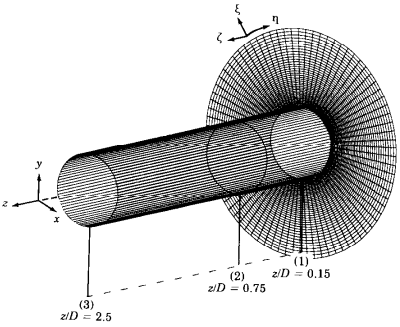
\includegraphics[width=1\linewidth]{graph_1}
			\caption{Three-dimensional grid}
			\label{fig:4_1}
		\end{minipage}
		\begin{minipage}{.3\textwidth}
			\centering
			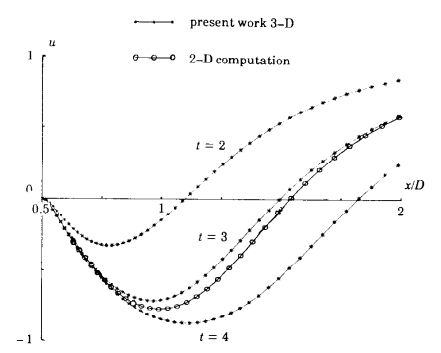
\includegraphics[width=1.3\linewidth]{graph_2}
			\caption{Evolution with time of the velocity profile; $R_e=200$}
			\label{fig:4_2}
		\end{minipage}
	\end{figure}

	\begin{figure}[!h]
		\centering
		\begin{minipage}{.4\textwidth}
			\centering
			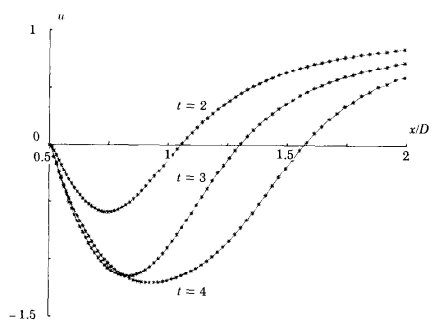
\includegraphics[width=1\linewidth]{graph_3}
			\caption{Evolution with time of the velocity profile; $R_e=100$}
			\label{fig:4_3}
		\end{minipage}
		\begin{minipage}{.3\textwidth}
			\centering
			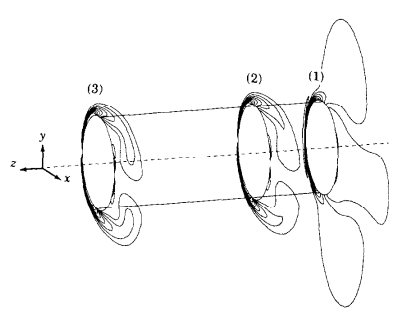
\includegraphics[width=1.3\linewidth]{graph_4}
			\caption{Vorticity contours in three cross sections; $\Delta\omega = 2, R_e=200, t=3$}
			\label{fig:4_4}
		\end{minipage}
	\end{figure}
	consists of 81 nodes in the radial $(\xi)$ direction, 81 in the azimuthal $(\eta)$ direction and 101 in the spanwise $(\zeta)$ direction, and for $R_e = 1000$ a grid system of $121 \times 121 \times 121$ nodes has been chosen.\\
	
	\NI Calculations were made on CRAY 2 and the computational cost is about $2 \cdot 1O^{-5}$ seconds per point and per time step to obtain a divergence norm less than $10^{-3}$. The dimensionless time step is 0.02 for $R_e = 200$ and 0.015 for $R_e = 1000$.\\
	The velocity profile time evolution behind the cylinder in the midspan section is reported in Fig. \ref{fig:4_2}. The Reynolds number is equal to 200. A comparison at time $t = 3$ with a 2-D computation obtained using a $\psi - \omega$ formulation reveals the two-dimensional behaviour in the central region of the flow.
	\begin{figure}[!h]
		\centering
		\begin{minipage}{.4\textwidth}
			\centering
			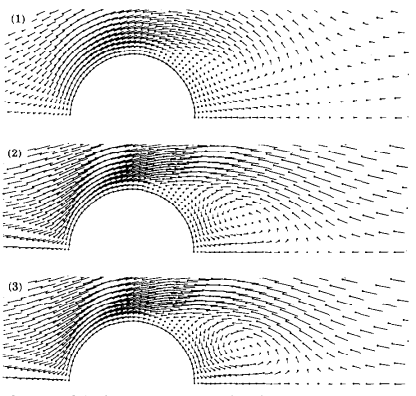
\includegraphics[width=1\linewidth]{graph_5}
			\caption{Velocity vectors plot in three cross sections; $R_e=200, t=3$}
			\label{fig:4_5}
		\end{minipage}
		\begin{minipage}{.4\textwidth}
			\centering
			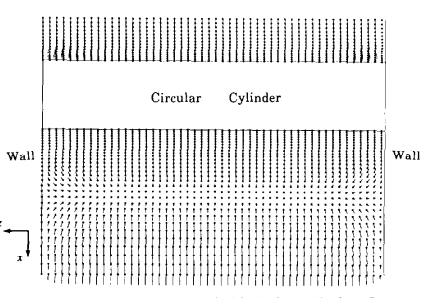
\includegraphics[width=1.3\linewidth]{graph_6}
			\caption{Velocity vectors plot behind the cylinder; $R_e=200, t=3$}
			\label{fig:4_6}
		\end{minipage}
	\end{figure}
	\begin{figure}[!h]
		\centering
		\begin{minipage}{.4\textwidth}
			\centering
			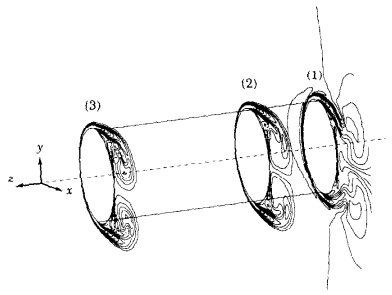
\includegraphics[width=1\linewidth]{graph_7}
			\caption{Vorticity contours in three cross sections; $\Delta\omega = 2, R_e=200, t=3$}
			\label{fig:4_7}
		\end{minipage}
		\begin{minipage}{.4\textwidth}
			\centering
			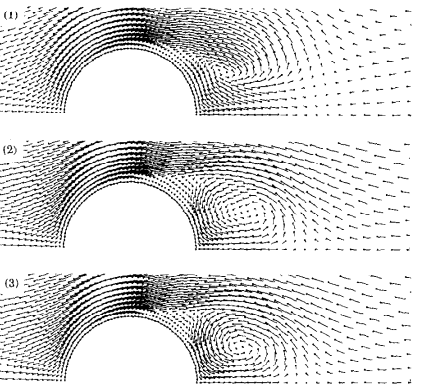
\includegraphics[width=1.3\linewidth]{graph_8}
			\caption{Vorticity contours in three cross sections; $\Delta\omega = 2, R_e=200, t=3$}
			\label{fig:4_8}
		\end{minipage}
	\end{figure}
	A similar curve for Re = 1000 is given in Fig. \ref{fig:4_3}. The length of the recirculating zone increases with time and is shorter for $R_e = 1000$ than for $R_e = 200$, in accordance with the results obtained in 2-D and in the experiments. We see that the peak of negative velocity increases with time and is more marked when the Reynolds number is greater.
	Figures \ref{fig:4_4}, \ref{fig:4_5} and \ref{fig:4_6} are related to a Reynolds number equal to 200 and Figs. \ref{fig:4_7} and \ref{fig:4_8} to a Reynolds number equal to 1000. 
	\\Figures \ref{fig:4_4} and \ref{fig:4_7} show the vorticity contours in three cross sections, the first plane is near the wall $(z/D = 0.15)$, the second one is intermediate $(s/D = 0.75)$ and the third one is the midspan section $(z/D = 2.5)$. \\
	Figures 5 and 8 show velocity vector plots in the same planes. Figure \ref{fig:4_6} shows velocity vectors plot behind the cylinder in the symmetric spanwise plane. For $R_e = 200$ a unique eddy is formed and for $R_e = 1000$ a secondary eddy appears.\\
	The three-dimensional effects are located especially near the walls, the different structures which appear in the flow are noticeably modified in these zones.
	
	
	
	
	
	%%%%%%%%%%%%%%%%%%%CHAPTER FIVE%%%%%%%%%%%%%%%%%%%
	\chapter{SUMMARY AND CONCLUSION}
	\section{Summary}
	
	
	\section{Conclusion}
	
	

	
	%%%%%%%%%%%%%%%%%%%REFERENCE%%%%%%%%%%%%%%%%%%%
	\chapter*{REFERENCES}
	\addcontentsline{toc}{chapter}{REFERENCES}
	
	\begin{description}
		\item 
	\end{description}
	
\end{document}